\documentclass{homeworg}

%\usepackage{amsmath, cancel, subcaption}
%\usepackage[shortlabels]{enumitem}
%\usepackage[export]{adjustbox}
%\usepackage[american, nooldvoltagedirection]{circuitikz}

%\usepackage{booktabs}
%%\usepackage{tabularx}
%\usepackage{multirow}

\usepackage{gnuplot-lua-tikz}
\usepackage{siunitx}
\usepackage{icomma}

\title{Materiais Elétricos e Magnéticos\\Tarefa 3}
\author{Matheus Henrique Wagner}
\date{Maio 2025}

\begin{document}

\maketitle

\begin{figure}[!h]
  \begin{minipage}{.49\linewidth}
    \centering
    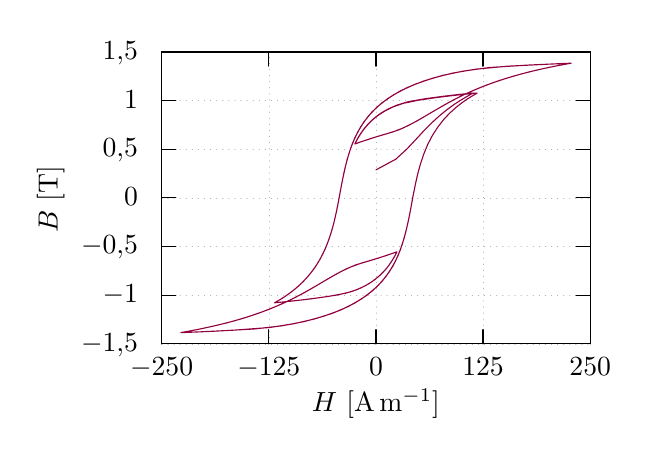
\begin{tikzpicture}[gnuplot]
%% generated with GNUPLOT 5.4p2 (Lua 5.4; terminal rev. Jun 2020, script rev. 114)
%% Fri 23 May 2025 09:04:49 AM -03
\path (0.000,0.000) rectangle (7.500,5.000);
\gpcolor{color=gp lt color axes}
\gpsetlinetype{gp lt axes}
\gpsetdashtype{gp dt axes}
\gpsetlinewidth{0.50}
\draw[gp path] (1.504,0.985)--(6.947,0.985);
\gpcolor{color=gp lt color border}
\gpsetlinetype{gp lt border}
\gpsetdashtype{gp dt solid}
\gpsetlinewidth{1.00}
\draw[gp path] (1.504,0.985)--(1.684,0.985);
\draw[gp path] (6.947,0.985)--(6.767,0.985);
\node[gp node right] at (1.320,0.985) {$-1,5$};
\gpcolor{color=gp lt color axes}
\gpsetlinetype{gp lt axes}
\gpsetdashtype{gp dt axes}
\gpsetlinewidth{0.50}
\draw[gp path] (1.504,1.603)--(6.947,1.603);
\gpcolor{color=gp lt color border}
\gpsetlinetype{gp lt border}
\gpsetdashtype{gp dt solid}
\gpsetlinewidth{1.00}
\draw[gp path] (1.504,1.603)--(1.684,1.603);
\draw[gp path] (6.947,1.603)--(6.767,1.603);
\node[gp node right] at (1.320,1.603) {$-1$};
\gpcolor{color=gp lt color axes}
\gpsetlinetype{gp lt axes}
\gpsetdashtype{gp dt axes}
\gpsetlinewidth{0.50}
\draw[gp path] (1.504,2.220)--(6.947,2.220);
\gpcolor{color=gp lt color border}
\gpsetlinetype{gp lt border}
\gpsetdashtype{gp dt solid}
\gpsetlinewidth{1.00}
\draw[gp path] (1.504,2.220)--(1.684,2.220);
\draw[gp path] (6.947,2.220)--(6.767,2.220);
\node[gp node right] at (1.320,2.220) {$-0,5$};
\gpcolor{color=gp lt color axes}
\gpsetlinetype{gp lt axes}
\gpsetdashtype{gp dt axes}
\gpsetlinewidth{0.50}
\draw[gp path] (1.504,2.838)--(6.947,2.838);
\gpcolor{color=gp lt color border}
\gpsetlinetype{gp lt border}
\gpsetdashtype{gp dt solid}
\gpsetlinewidth{1.00}
\draw[gp path] (1.504,2.838)--(1.684,2.838);
\draw[gp path] (6.947,2.838)--(6.767,2.838);
\node[gp node right] at (1.320,2.838) {$0$};
\gpcolor{color=gp lt color axes}
\gpsetlinetype{gp lt axes}
\gpsetdashtype{gp dt axes}
\gpsetlinewidth{0.50}
\draw[gp path] (1.504,3.456)--(6.947,3.456);
\gpcolor{color=gp lt color border}
\gpsetlinetype{gp lt border}
\gpsetdashtype{gp dt solid}
\gpsetlinewidth{1.00}
\draw[gp path] (1.504,3.456)--(1.684,3.456);
\draw[gp path] (6.947,3.456)--(6.767,3.456);
\node[gp node right] at (1.320,3.456) {$0,5$};
\gpcolor{color=gp lt color axes}
\gpsetlinetype{gp lt axes}
\gpsetdashtype{gp dt axes}
\gpsetlinewidth{0.50}
\draw[gp path] (1.504,4.073)--(6.947,4.073);
\gpcolor{color=gp lt color border}
\gpsetlinetype{gp lt border}
\gpsetdashtype{gp dt solid}
\gpsetlinewidth{1.00}
\draw[gp path] (1.504,4.073)--(1.684,4.073);
\draw[gp path] (6.947,4.073)--(6.767,4.073);
\node[gp node right] at (1.320,4.073) {$1$};
\gpcolor{color=gp lt color axes}
\gpsetlinetype{gp lt axes}
\gpsetdashtype{gp dt axes}
\gpsetlinewidth{0.50}
\draw[gp path] (1.504,4.691)--(6.947,4.691);
\gpcolor{color=gp lt color border}
\gpsetlinetype{gp lt border}
\gpsetdashtype{gp dt solid}
\gpsetlinewidth{1.00}
\draw[gp path] (1.504,4.691)--(1.684,4.691);
\draw[gp path] (6.947,4.691)--(6.767,4.691);
\node[gp node right] at (1.320,4.691) {$1,5$};
\gpcolor{color=gp lt color axes}
\gpsetlinetype{gp lt axes}
\gpsetdashtype{gp dt axes}
\gpsetlinewidth{0.50}
\draw[gp path] (1.504,0.985)--(1.504,4.691);
\gpcolor{color=gp lt color border}
\gpsetlinetype{gp lt border}
\gpsetdashtype{gp dt solid}
\gpsetlinewidth{1.00}
\draw[gp path] (1.504,0.985)--(1.504,1.165);
\draw[gp path] (1.504,4.691)--(1.504,4.511);
\node[gp node center] at (1.504,0.677) {$-250$};
\gpcolor{color=gp lt color axes}
\gpsetlinetype{gp lt axes}
\gpsetdashtype{gp dt axes}
\gpsetlinewidth{0.50}
\draw[gp path] (2.865,0.985)--(2.865,4.691);
\gpcolor{color=gp lt color border}
\gpsetlinetype{gp lt border}
\gpsetdashtype{gp dt solid}
\gpsetlinewidth{1.00}
\draw[gp path] (2.865,0.985)--(2.865,1.165);
\draw[gp path] (2.865,4.691)--(2.865,4.511);
\node[gp node center] at (2.865,0.677) {$-125$};
\gpcolor{color=gp lt color axes}
\gpsetlinetype{gp lt axes}
\gpsetdashtype{gp dt axes}
\gpsetlinewidth{0.50}
\draw[gp path] (4.226,0.985)--(4.226,4.691);
\gpcolor{color=gp lt color border}
\gpsetlinetype{gp lt border}
\gpsetdashtype{gp dt solid}
\gpsetlinewidth{1.00}
\draw[gp path] (4.226,0.985)--(4.226,1.165);
\draw[gp path] (4.226,4.691)--(4.226,4.511);
\node[gp node center] at (4.226,0.677) {$0$};
\gpcolor{color=gp lt color axes}
\gpsetlinetype{gp lt axes}
\gpsetdashtype{gp dt axes}
\gpsetlinewidth{0.50}
\draw[gp path] (5.586,0.985)--(5.586,4.691);
\gpcolor{color=gp lt color border}
\gpsetlinetype{gp lt border}
\gpsetdashtype{gp dt solid}
\gpsetlinewidth{1.00}
\draw[gp path] (5.586,0.985)--(5.586,1.165);
\draw[gp path] (5.586,4.691)--(5.586,4.511);
\node[gp node center] at (5.586,0.677) {$125$};
\gpcolor{color=gp lt color axes}
\gpsetlinetype{gp lt axes}
\gpsetdashtype{gp dt axes}
\gpsetlinewidth{0.50}
\draw[gp path] (6.947,0.985)--(6.947,4.691);
\gpcolor{color=gp lt color border}
\gpsetlinetype{gp lt border}
\gpsetdashtype{gp dt solid}
\gpsetlinewidth{1.00}
\draw[gp path] (6.947,0.985)--(6.947,1.165);
\draw[gp path] (6.947,4.691)--(6.947,4.511);
\node[gp node center] at (6.947,0.677) {$250$};
\draw[gp path] (1.504,4.691)--(1.504,0.985)--(6.947,0.985)--(6.947,4.691)--cycle;
\node[gp node center,rotate=-270] at (0.108,2.838) {$B$ [\si{\tesla}]};
\node[gp node center] at (4.225,0.215) {$H$ [\si{\ampere\per\meter}]};
\gpcolor{rgb color={0.569,0.000,0.247}}
\draw[gp path] (4.226,3.194)--(4.477,3.329)--(4.617,3.457)--(4.729,3.576)--(4.831,3.687)%
  --(4.930,3.787)--(5.027,3.876)--(5.122,3.954)--(5.212,4.020)--(5.294,4.074)--(5.364,4.116)%
  --(5.417,4.146)--(5.450,4.164)--(5.463,4.170)--(5.419,4.166)--(5.282,4.152)--(5.083,4.129)%
  --(4.854,4.098)--(4.636,4.060)--(4.491,4.016)--(4.382,3.968)--(4.294,3.918)--(4.222,3.865)%
  --(4.162,3.813)--(4.113,3.761)--(4.072,3.712)--(4.040,3.667)--(4.013,3.626)--(3.992,3.590)%
  --(3.977,3.562)--(3.966,3.541)--(3.960,3.528)--(3.957,3.523)--(3.969,3.527)--(4.005,3.540)%
  --(4.068,3.561)--(4.159,3.592)--(4.284,3.630)--(4.442,3.676)--(4.577,3.728)--(4.694,3.787)%
  --(4.807,3.850)--(4.921,3.918)--(5.040,3.987)--(5.167,4.059)--(5.304,4.130)--(5.454,4.199)%
  --(5.617,4.266)--(5.793,4.329)--(5.978,4.386)--(6.166,4.437)--(6.347,4.479)--(6.506,4.512)%
  --(6.628,4.535)--(6.696,4.547)--(6.670,4.547)--(6.384,4.535)--(5.902,4.511)--(5.492,4.473)%
  --(5.199,4.423)--(4.947,4.359)--(4.726,4.283)--(4.534,4.196)--(4.371,4.097)--(4.234,3.987)%
  --(4.122,3.868)--(4.032,3.741)--(3.960,3.606)--(3.904,3.466)--(3.859,3.322)--(3.823,3.174)%
  --(3.793,3.026)--(3.765,2.877)--(3.738,2.730)--(3.707,2.586)--(3.672,2.447)--(3.630,2.314)%
  --(3.581,2.189)--(3.523,2.071)--(3.457,1.963)--(3.384,1.866)--(3.306,1.779)--(3.226,1.704)%
  --(3.148,1.641)--(3.076,1.590)--(3.016,1.551)--(2.971,1.525)--(2.945,1.510)--(2.939,1.506)%
  --(3.011,1.513)--(3.171,1.529)--(3.386,1.554)--(3.623,1.587)--(3.839,1.627)--(3.980,1.671)%
  --(4.086,1.720)--(4.171,1.771)--(4.241,1.824)--(4.299,1.876)--(4.347,1.927)--(4.386,1.976)%
  --(4.417,2.020)--(4.442,2.060)--(4.462,2.093)--(4.476,2.120)--(4.486,2.139)--(4.491,2.150)%
  --(4.492,2.153)--(4.474,2.147)--(4.431,2.132)--(4.362,2.108)--(4.262,2.076)--(4.129,2.035)%
  --(3.971,1.988)--(3.843,1.934)--(3.728,1.874)--(3.615,1.809)--(3.500,1.741)--(3.380,1.671)%
  --(3.251,1.600)--(3.110,1.529)--(2.957,1.460)--(2.791,1.394)--(2.613,1.332)--(2.426,1.276)%
  --(2.239,1.228)--(2.062,1.188)--(1.910,1.157)--(1.800,1.137)--(1.748,1.128)--(1.827,1.130)%
  --(2.174,1.145)--(2.678,1.173)--(3.037,1.214)--(3.318,1.268)--(3.562,1.335)--(3.776,1.413)%
  --(3.960,1.504)--(4.117,1.606)--(4.247,1.718)--(4.353,1.839)--(4.439,1.968)--(4.506,2.104)%
  --(4.559,2.246)--(4.601,2.391)--(4.636,2.539)--(4.665,2.688)--(4.692,2.836)--(4.721,2.982)%
  --(4.752,3.125)--(4.789,3.262)--(4.833,3.394)--(4.884,3.518)--(4.944,3.633)--(5.012,3.738)%
  --(5.086,3.833)--(5.165,3.917)--(5.245,3.989)--(5.322,4.049)--(5.391,4.097)--(5.448,4.132)%
  --(5.488,4.156)--(5.510,4.168)--(5.504,4.169)--(5.407,4.160)--(5.230,4.141)--(5.006,4.114)%
  --(4.768,4.079)--(4.572,4.039)--(4.442,3.993)--(4.342,3.943)--(4.261,3.892)--(4.194,3.839)%
  --(4.139,3.787)--(4.094,3.736)--(4.057,3.689)--(4.027,3.645)--(4.004,3.607)--(3.985,3.575)%
  --(3.972,3.550)--(3.963,3.533)--(3.959,3.524)--(3.961,3.524)--(3.985,3.532)--(4.034,3.550)%
  --(4.111,3.575)--(4.218,3.610)--(4.361,3.652)--(4.514,3.701)--(4.637,3.757)--(4.751,3.818)%
  --(4.864,3.884)--(4.980,3.952)--(5.102,4.023)--(5.234,4.094)--(5.378,4.165)--(5.534,4.233)%
  --(5.704,4.298)--(5.884,4.358)--(6.072,4.412)--(6.258,4.459)--(6.430,4.497)--(6.573,4.525)%
  --(6.670,4.543)--(6.706,4.549)--(6.560,4.543)--(6.159,4.525)--(5.668,4.494)--(5.339,4.449)%
  --(5.069,4.393)--(4.833,4.323)--(4.626,4.241)--(4.449,4.147)--(4.299,4.043)--(4.175,3.929)%
  --(4.074,3.805)--(3.994,3.674)--(3.930,3.537)--(3.880,3.394)--(3.841,3.248)--(3.808,3.100)%
  --(3.779,2.951)--(3.752,2.803)--(3.723,2.658)--(3.690,2.516)--(3.652,2.380)--(3.606,2.250)%
  --(3.553,2.129)--(3.491,2.016)--(3.421,1.913)--(3.345,1.821)--(3.266,1.740)--(3.186,1.671)%
  --(3.111,1.614)--(3.045,1.569)--(2.992,1.537)--(2.956,1.516)--(2.939,1.507)--(2.962,1.508)%
  --(3.082,1.520)--(3.274,1.541)--(3.504,1.570)--(3.742,1.606)--(3.916,1.648)--(4.036,1.695)%
  --(4.131,1.745)--(4.208,1.797)--(4.272,1.850)--(4.324,1.902)--(4.367,1.952)--(4.402,1.998)%
  --(4.430,2.041)--(4.452,2.077)--(4.469,2.108)--(4.481,2.131)--(4.489,2.146)--(4.492,2.153)%
  --(4.486,2.151)--(4.456,2.140)--(4.400,2.121)--(4.316,2.093)--(4.200,2.056)--(4.047,2.012)%
  --(3.905,1.961)--(3.785,1.904)--(3.672,1.842)--(3.559,1.776)--(3.441,1.706)--(3.317,1.635)%
  --(3.182,1.564)--(3.036,1.494)--(2.876,1.426)--(2.703,1.362)--(2.520,1.303)--(2.332,1.251)%
  --(2.148,1.207)--(1.982,1.171)--(1.849,1.146)--(1.766,1.131)--(1.753,1.127)--(1.972,1.136)%
  --(2.417,1.158)--(2.875,1.192)--(3.184,1.240)--(3.444,1.300)--(3.673,1.372)--(3.872,1.457)%
  --(4.042,1.554)--(4.185,1.661)--(4.303,1.777)--(4.398,1.903)--(4.474,2.035)--(4.534,2.174)%
  --(4.581,2.318)--(4.619,2.465)--(4.651,2.613)--(4.679,2.762)--(4.706,2.909)--(4.736,3.054)%
  --(4.770,3.194);
\gpcolor{color=gp lt color border}
\draw[gp path] (1.504,4.691)--(1.504,0.985)--(6.947,0.985)--(6.947,4.691)--cycle;
%% coordinates of the plot area
\gpdefrectangularnode{gp plot 1}{\pgfpoint{1.504cm}{0.985cm}}{\pgfpoint{6.947cm}{4.691cm}}
\end{tikzpicture}
%% gnuplot variables

    \vspace{-1cm}
    \caption{uma caption}
  \end{minipage}%
  \begin{minipage}{.49\linewidth}
    \centering
    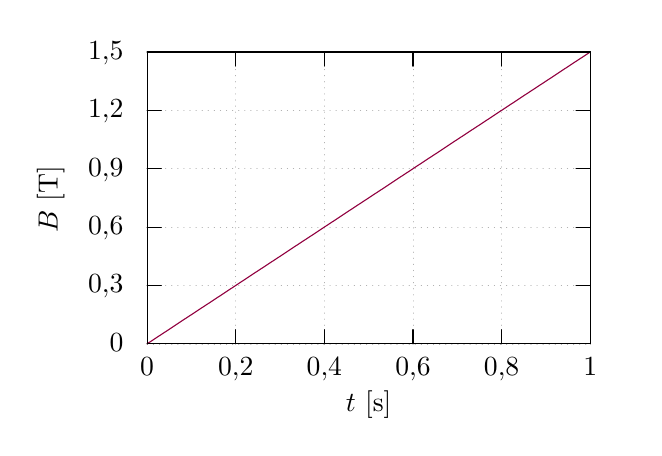
\begin{tikzpicture}[gnuplot]
%% generated with GNUPLOT 5.4p2 (Lua 5.4; terminal rev. Jun 2020, script rev. 114)
%% Fri 23 May 2025 09:06:32 AM -03
\path (0.000,0.000) rectangle (7.500,5.000);
\gpcolor{color=gp lt color axes}
\gpsetlinetype{gp lt axes}
\gpsetdashtype{gp dt axes}
\gpsetlinewidth{0.50}
\draw[gp path] (1.320,0.985)--(6.947,0.985);
\gpcolor{color=gp lt color border}
\gpsetlinetype{gp lt border}
\gpsetdashtype{gp dt solid}
\gpsetlinewidth{1.00}
\draw[gp path] (1.320,0.985)--(1.500,0.985);
\draw[gp path] (6.947,0.985)--(6.767,0.985);
\node[gp node right] at (1.136,0.985) {$0$};
\gpcolor{color=gp lt color axes}
\gpsetlinetype{gp lt axes}
\gpsetdashtype{gp dt axes}
\gpsetlinewidth{0.50}
\draw[gp path] (1.320,1.726)--(6.947,1.726);
\gpcolor{color=gp lt color border}
\gpsetlinetype{gp lt border}
\gpsetdashtype{gp dt solid}
\gpsetlinewidth{1.00}
\draw[gp path] (1.320,1.726)--(1.500,1.726);
\draw[gp path] (6.947,1.726)--(6.767,1.726);
\node[gp node right] at (1.136,1.726) {$0,3$};
\gpcolor{color=gp lt color axes}
\gpsetlinetype{gp lt axes}
\gpsetdashtype{gp dt axes}
\gpsetlinewidth{0.50}
\draw[gp path] (1.320,2.467)--(6.947,2.467);
\gpcolor{color=gp lt color border}
\gpsetlinetype{gp lt border}
\gpsetdashtype{gp dt solid}
\gpsetlinewidth{1.00}
\draw[gp path] (1.320,2.467)--(1.500,2.467);
\draw[gp path] (6.947,2.467)--(6.767,2.467);
\node[gp node right] at (1.136,2.467) {$0,6$};
\gpcolor{color=gp lt color axes}
\gpsetlinetype{gp lt axes}
\gpsetdashtype{gp dt axes}
\gpsetlinewidth{0.50}
\draw[gp path] (1.320,3.209)--(6.947,3.209);
\gpcolor{color=gp lt color border}
\gpsetlinetype{gp lt border}
\gpsetdashtype{gp dt solid}
\gpsetlinewidth{1.00}
\draw[gp path] (1.320,3.209)--(1.500,3.209);
\draw[gp path] (6.947,3.209)--(6.767,3.209);
\node[gp node right] at (1.136,3.209) {$0,9$};
\gpcolor{color=gp lt color axes}
\gpsetlinetype{gp lt axes}
\gpsetdashtype{gp dt axes}
\gpsetlinewidth{0.50}
\draw[gp path] (1.320,3.950)--(6.947,3.950);
\gpcolor{color=gp lt color border}
\gpsetlinetype{gp lt border}
\gpsetdashtype{gp dt solid}
\gpsetlinewidth{1.00}
\draw[gp path] (1.320,3.950)--(1.500,3.950);
\draw[gp path] (6.947,3.950)--(6.767,3.950);
\node[gp node right] at (1.136,3.950) {$1,2$};
\gpcolor{color=gp lt color axes}
\gpsetlinetype{gp lt axes}
\gpsetdashtype{gp dt axes}
\gpsetlinewidth{0.50}
\draw[gp path] (1.320,4.691)--(6.947,4.691);
\gpcolor{color=gp lt color border}
\gpsetlinetype{gp lt border}
\gpsetdashtype{gp dt solid}
\gpsetlinewidth{1.00}
\draw[gp path] (1.320,4.691)--(1.500,4.691);
\draw[gp path] (6.947,4.691)--(6.767,4.691);
\node[gp node right] at (1.136,4.691) {$1,5$};
\gpcolor{color=gp lt color axes}
\gpsetlinetype{gp lt axes}
\gpsetdashtype{gp dt axes}
\gpsetlinewidth{0.50}
\draw[gp path] (1.320,0.985)--(1.320,4.691);
\gpcolor{color=gp lt color border}
\gpsetlinetype{gp lt border}
\gpsetdashtype{gp dt solid}
\gpsetlinewidth{1.00}
\draw[gp path] (1.320,0.985)--(1.320,1.165);
\draw[gp path] (1.320,4.691)--(1.320,4.511);
\node[gp node center] at (1.320,0.677) {$0$};
\gpcolor{color=gp lt color axes}
\gpsetlinetype{gp lt axes}
\gpsetdashtype{gp dt axes}
\gpsetlinewidth{0.50}
\draw[gp path] (2.445,0.985)--(2.445,4.691);
\gpcolor{color=gp lt color border}
\gpsetlinetype{gp lt border}
\gpsetdashtype{gp dt solid}
\gpsetlinewidth{1.00}
\draw[gp path] (2.445,0.985)--(2.445,1.165);
\draw[gp path] (2.445,4.691)--(2.445,4.511);
\node[gp node center] at (2.445,0.677) {$0,2$};
\gpcolor{color=gp lt color axes}
\gpsetlinetype{gp lt axes}
\gpsetdashtype{gp dt axes}
\gpsetlinewidth{0.50}
\draw[gp path] (3.571,0.985)--(3.571,4.691);
\gpcolor{color=gp lt color border}
\gpsetlinetype{gp lt border}
\gpsetdashtype{gp dt solid}
\gpsetlinewidth{1.00}
\draw[gp path] (3.571,0.985)--(3.571,1.165);
\draw[gp path] (3.571,4.691)--(3.571,4.511);
\node[gp node center] at (3.571,0.677) {$0,4$};
\gpcolor{color=gp lt color axes}
\gpsetlinetype{gp lt axes}
\gpsetdashtype{gp dt axes}
\gpsetlinewidth{0.50}
\draw[gp path] (4.696,0.985)--(4.696,4.691);
\gpcolor{color=gp lt color border}
\gpsetlinetype{gp lt border}
\gpsetdashtype{gp dt solid}
\gpsetlinewidth{1.00}
\draw[gp path] (4.696,0.985)--(4.696,1.165);
\draw[gp path] (4.696,4.691)--(4.696,4.511);
\node[gp node center] at (4.696,0.677) {$0,6$};
\gpcolor{color=gp lt color axes}
\gpsetlinetype{gp lt axes}
\gpsetdashtype{gp dt axes}
\gpsetlinewidth{0.50}
\draw[gp path] (5.822,0.985)--(5.822,4.691);
\gpcolor{color=gp lt color border}
\gpsetlinetype{gp lt border}
\gpsetdashtype{gp dt solid}
\gpsetlinewidth{1.00}
\draw[gp path] (5.822,0.985)--(5.822,1.165);
\draw[gp path] (5.822,4.691)--(5.822,4.511);
\node[gp node center] at (5.822,0.677) {$0,8$};
\gpcolor{color=gp lt color axes}
\gpsetlinetype{gp lt axes}
\gpsetdashtype{gp dt axes}
\gpsetlinewidth{0.50}
\draw[gp path] (6.947,0.985)--(6.947,4.691);
\gpcolor{color=gp lt color border}
\gpsetlinetype{gp lt border}
\gpsetdashtype{gp dt solid}
\gpsetlinewidth{1.00}
\draw[gp path] (6.947,0.985)--(6.947,1.165);
\draw[gp path] (6.947,4.691)--(6.947,4.511);
\node[gp node center] at (6.947,0.677) {$1$};
\draw[gp path] (1.320,4.691)--(1.320,0.985)--(6.947,0.985)--(6.947,4.691)--cycle;
\node[gp node center,rotate=-270] at (0.108,2.838) {$B$ [\si{\tesla}]};
\node[gp node center] at (4.133,0.215) {$t$ [\si{\second}]};
\gpcolor{rgb color={0.569,0.000,0.247}}
\draw[gp path] (1.320,0.985)--(1.435,1.061)--(1.550,1.136)--(1.665,1.212)--(1.779,1.288)%
  --(1.894,1.363)--(2.009,1.439)--(2.124,1.514)--(2.239,1.590)--(2.354,1.666)--(2.468,1.741)%
  --(2.583,1.817)--(2.698,1.893)--(2.813,1.968)--(2.928,2.044)--(3.043,2.119)--(3.157,2.195)%
  --(3.272,2.271)--(3.387,2.346)--(3.502,2.422)--(3.617,2.498)--(3.732,2.573)--(3.846,2.649)%
  --(3.961,2.725)--(4.076,2.800)--(4.191,2.876)--(4.306,2.951)--(4.421,3.027)--(4.535,3.103)%
  --(4.650,3.178)--(4.765,3.254)--(4.880,3.330)--(4.995,3.405)--(5.110,3.481)--(5.224,3.557)%
  --(5.339,3.632)--(5.454,3.708)--(5.569,3.783)--(5.684,3.859)--(5.799,3.935)--(5.913,4.010)%
  --(6.028,4.086)--(6.143,4.162)--(6.258,4.237)--(6.373,4.313)--(6.488,4.388)--(6.602,4.464)%
  --(6.717,4.540)--(6.832,4.615)--(6.947,4.691);
\gpcolor{color=gp lt color border}
\draw[gp path] (1.320,4.691)--(1.320,0.985)--(6.947,0.985)--(6.947,4.691)--cycle;
%% coordinates of the plot area
\gpdefrectangularnode{gp plot 1}{\pgfpoint{1.320cm}{0.985cm}}{\pgfpoint{6.947cm}{4.691cm}}
\end{tikzpicture}
%% gnuplot variables

    \vspace{-1cm}
    \caption{HHHHHHHHHHHHHHH}
  \end{minipage}
  \begin{minipage}{.49\linewidth}
    \centering
    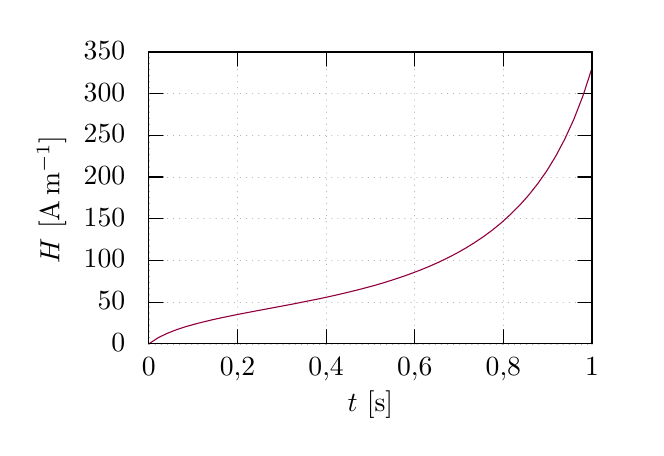
\begin{tikzpicture}[gnuplot]
%% generated with GNUPLOT 5.4p2 (Lua 5.4; terminal rev. Jun 2020, script rev. 114)
%% Fri 23 May 2025 09:06:32 AM -03
\path (0.000,0.000) rectangle (7.500,5.000);
\gpcolor{color=gp lt color axes}
\gpsetlinetype{gp lt axes}
\gpsetdashtype{gp dt axes}
\gpsetlinewidth{0.50}
\draw[gp path] (1.320,0.985)--(6.947,0.985);
\gpcolor{color=gp lt color border}
\gpsetlinetype{gp lt border}
\gpsetdashtype{gp dt solid}
\gpsetlinewidth{1.00}
\draw[gp path] (1.320,0.985)--(1.500,0.985);
\draw[gp path] (6.947,0.985)--(6.767,0.985);
\node[gp node right] at (1.136,0.985) {$0$};
\gpcolor{color=gp lt color axes}
\gpsetlinetype{gp lt axes}
\gpsetdashtype{gp dt axes}
\gpsetlinewidth{0.50}
\draw[gp path] (1.320,1.514)--(6.947,1.514);
\gpcolor{color=gp lt color border}
\gpsetlinetype{gp lt border}
\gpsetdashtype{gp dt solid}
\gpsetlinewidth{1.00}
\draw[gp path] (1.320,1.514)--(1.500,1.514);
\draw[gp path] (6.947,1.514)--(6.767,1.514);
\node[gp node right] at (1.136,1.514) {$50$};
\gpcolor{color=gp lt color axes}
\gpsetlinetype{gp lt axes}
\gpsetdashtype{gp dt axes}
\gpsetlinewidth{0.50}
\draw[gp path] (1.320,2.044)--(6.947,2.044);
\gpcolor{color=gp lt color border}
\gpsetlinetype{gp lt border}
\gpsetdashtype{gp dt solid}
\gpsetlinewidth{1.00}
\draw[gp path] (1.320,2.044)--(1.500,2.044);
\draw[gp path] (6.947,2.044)--(6.767,2.044);
\node[gp node right] at (1.136,2.044) {$100$};
\gpcolor{color=gp lt color axes}
\gpsetlinetype{gp lt axes}
\gpsetdashtype{gp dt axes}
\gpsetlinewidth{0.50}
\draw[gp path] (1.320,2.573)--(6.947,2.573);
\gpcolor{color=gp lt color border}
\gpsetlinetype{gp lt border}
\gpsetdashtype{gp dt solid}
\gpsetlinewidth{1.00}
\draw[gp path] (1.320,2.573)--(1.500,2.573);
\draw[gp path] (6.947,2.573)--(6.767,2.573);
\node[gp node right] at (1.136,2.573) {$150$};
\gpcolor{color=gp lt color axes}
\gpsetlinetype{gp lt axes}
\gpsetdashtype{gp dt axes}
\gpsetlinewidth{0.50}
\draw[gp path] (1.320,3.103)--(6.947,3.103);
\gpcolor{color=gp lt color border}
\gpsetlinetype{gp lt border}
\gpsetdashtype{gp dt solid}
\gpsetlinewidth{1.00}
\draw[gp path] (1.320,3.103)--(1.500,3.103);
\draw[gp path] (6.947,3.103)--(6.767,3.103);
\node[gp node right] at (1.136,3.103) {$200$};
\gpcolor{color=gp lt color axes}
\gpsetlinetype{gp lt axes}
\gpsetdashtype{gp dt axes}
\gpsetlinewidth{0.50}
\draw[gp path] (1.320,3.632)--(6.947,3.632);
\gpcolor{color=gp lt color border}
\gpsetlinetype{gp lt border}
\gpsetdashtype{gp dt solid}
\gpsetlinewidth{1.00}
\draw[gp path] (1.320,3.632)--(1.500,3.632);
\draw[gp path] (6.947,3.632)--(6.767,3.632);
\node[gp node right] at (1.136,3.632) {$250$};
\gpcolor{color=gp lt color axes}
\gpsetlinetype{gp lt axes}
\gpsetdashtype{gp dt axes}
\gpsetlinewidth{0.50}
\draw[gp path] (1.320,4.162)--(6.947,4.162);
\gpcolor{color=gp lt color border}
\gpsetlinetype{gp lt border}
\gpsetdashtype{gp dt solid}
\gpsetlinewidth{1.00}
\draw[gp path] (1.320,4.162)--(1.500,4.162);
\draw[gp path] (6.947,4.162)--(6.767,4.162);
\node[gp node right] at (1.136,4.162) {$300$};
\gpcolor{color=gp lt color axes}
\gpsetlinetype{gp lt axes}
\gpsetdashtype{gp dt axes}
\gpsetlinewidth{0.50}
\draw[gp path] (1.320,4.691)--(6.947,4.691);
\gpcolor{color=gp lt color border}
\gpsetlinetype{gp lt border}
\gpsetdashtype{gp dt solid}
\gpsetlinewidth{1.00}
\draw[gp path] (1.320,4.691)--(1.500,4.691);
\draw[gp path] (6.947,4.691)--(6.767,4.691);
\node[gp node right] at (1.136,4.691) {$350$};
\gpcolor{color=gp lt color axes}
\gpsetlinetype{gp lt axes}
\gpsetdashtype{gp dt axes}
\gpsetlinewidth{0.50}
\draw[gp path] (1.320,0.985)--(1.320,4.691);
\gpcolor{color=gp lt color border}
\gpsetlinetype{gp lt border}
\gpsetdashtype{gp dt solid}
\gpsetlinewidth{1.00}
\draw[gp path] (1.320,0.985)--(1.320,1.165);
\draw[gp path] (1.320,4.691)--(1.320,4.511);
\node[gp node center] at (1.320,0.677) {$0$};
\gpcolor{color=gp lt color axes}
\gpsetlinetype{gp lt axes}
\gpsetdashtype{gp dt axes}
\gpsetlinewidth{0.50}
\draw[gp path] (2.445,0.985)--(2.445,4.691);
\gpcolor{color=gp lt color border}
\gpsetlinetype{gp lt border}
\gpsetdashtype{gp dt solid}
\gpsetlinewidth{1.00}
\draw[gp path] (2.445,0.985)--(2.445,1.165);
\draw[gp path] (2.445,4.691)--(2.445,4.511);
\node[gp node center] at (2.445,0.677) {$0,2$};
\gpcolor{color=gp lt color axes}
\gpsetlinetype{gp lt axes}
\gpsetdashtype{gp dt axes}
\gpsetlinewidth{0.50}
\draw[gp path] (3.571,0.985)--(3.571,4.691);
\gpcolor{color=gp lt color border}
\gpsetlinetype{gp lt border}
\gpsetdashtype{gp dt solid}
\gpsetlinewidth{1.00}
\draw[gp path] (3.571,0.985)--(3.571,1.165);
\draw[gp path] (3.571,4.691)--(3.571,4.511);
\node[gp node center] at (3.571,0.677) {$0,4$};
\gpcolor{color=gp lt color axes}
\gpsetlinetype{gp lt axes}
\gpsetdashtype{gp dt axes}
\gpsetlinewidth{0.50}
\draw[gp path] (4.696,0.985)--(4.696,4.691);
\gpcolor{color=gp lt color border}
\gpsetlinetype{gp lt border}
\gpsetdashtype{gp dt solid}
\gpsetlinewidth{1.00}
\draw[gp path] (4.696,0.985)--(4.696,1.165);
\draw[gp path] (4.696,4.691)--(4.696,4.511);
\node[gp node center] at (4.696,0.677) {$0,6$};
\gpcolor{color=gp lt color axes}
\gpsetlinetype{gp lt axes}
\gpsetdashtype{gp dt axes}
\gpsetlinewidth{0.50}
\draw[gp path] (5.822,0.985)--(5.822,4.691);
\gpcolor{color=gp lt color border}
\gpsetlinetype{gp lt border}
\gpsetdashtype{gp dt solid}
\gpsetlinewidth{1.00}
\draw[gp path] (5.822,0.985)--(5.822,1.165);
\draw[gp path] (5.822,4.691)--(5.822,4.511);
\node[gp node center] at (5.822,0.677) {$0,8$};
\gpcolor{color=gp lt color axes}
\gpsetlinetype{gp lt axes}
\gpsetdashtype{gp dt axes}
\gpsetlinewidth{0.50}
\draw[gp path] (6.947,0.985)--(6.947,4.691);
\gpcolor{color=gp lt color border}
\gpsetlinetype{gp lt border}
\gpsetdashtype{gp dt solid}
\gpsetlinewidth{1.00}
\draw[gp path] (6.947,0.985)--(6.947,1.165);
\draw[gp path] (6.947,4.691)--(6.947,4.511);
\node[gp node center] at (6.947,0.677) {$1$};
\draw[gp path] (1.320,4.691)--(1.320,0.985)--(6.947,0.985)--(6.947,4.691)--cycle;
\node[gp node center,rotate=-270] at (0.108,2.838) {$H$ [\si{\ampere\per\meter}]};
\node[gp node center] at (4.133,0.215) {$t$ [\si{\second}]};
\gpcolor{rgb color={0.569,0.000,0.247}}
\draw[gp path] (1.320,0.985)--(1.435,1.061)--(1.550,1.117)--(1.665,1.162)--(1.779,1.200)%
  --(1.894,1.233)--(2.009,1.262)--(2.124,1.290)--(2.239,1.315)--(2.354,1.339)--(2.468,1.362)%
  --(2.583,1.384)--(2.698,1.406)--(2.813,1.427)--(2.928,1.449)--(3.043,1.470)--(3.157,1.492)%
  --(3.272,1.515)--(3.387,1.538)--(3.502,1.561)--(3.617,1.586)--(3.732,1.612)--(3.846,1.639)%
  --(3.961,1.667)--(4.076,1.697)--(4.191,1.728)--(4.306,1.762)--(4.421,1.798)--(4.535,1.836)%
  --(4.650,1.877)--(4.765,1.921)--(4.880,1.968)--(4.995,2.019)--(5.110,2.074)--(5.224,2.133)%
  --(5.339,2.198)--(5.454,2.269)--(5.569,2.346)--(5.684,2.431)--(5.799,2.525)--(5.913,2.629)%
  --(6.028,2.744)--(6.143,2.873)--(6.258,3.018)--(6.373,3.182)--(6.488,3.370)--(6.602,3.586)%
  --(6.717,3.837)--(6.832,4.133)--(6.947,4.486);
\gpcolor{color=gp lt color border}
\draw[gp path] (1.320,4.691)--(1.320,0.985)--(6.947,0.985)--(6.947,4.691)--cycle;
%% coordinates of the plot area
\gpdefrectangularnode{gp plot 1}{\pgfpoint{1.320cm}{0.985cm}}{\pgfpoint{6.947cm}{4.691cm}}
\end{tikzpicture}
%% gnuplot variables

    \vspace{-1cm}
    \caption{uma caption}
  \end{minipage}%
  \begin{minipage}{.49\linewidth}
    \centering
    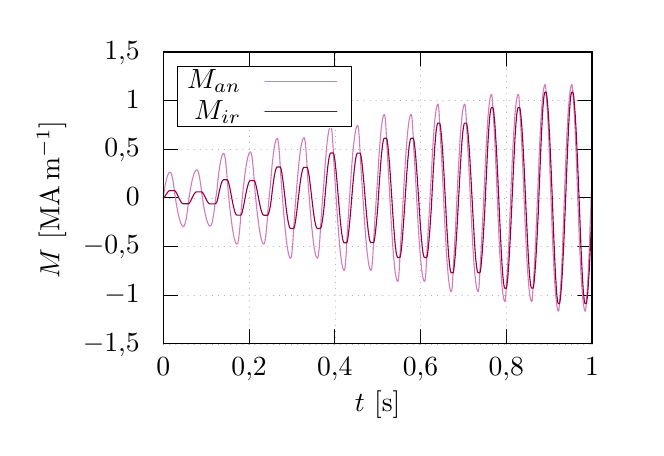
\begin{tikzpicture}[gnuplot]
%% generated with GNUPLOT 5.4p2 (Lua 5.4; terminal rev. Jun 2020, script rev. 114)
%% Fri 23 May 2025 09:05:47 AM -03
\path (0.000,0.000) rectangle (7.500,5.000);
\gpcolor{color=gp lt color axes}
\gpsetlinetype{gp lt axes}
\gpsetdashtype{gp dt axes}
\gpsetlinewidth{0.50}
\draw[gp path] (1.504,0.985)--(6.947,0.985);
\gpcolor{color=gp lt color border}
\gpsetlinetype{gp lt border}
\gpsetdashtype{gp dt solid}
\gpsetlinewidth{1.00}
\draw[gp path] (1.504,0.985)--(1.684,0.985);
\draw[gp path] (6.947,0.985)--(6.767,0.985);
\node[gp node right] at (1.320,0.985) {$-1,5$};
\gpcolor{color=gp lt color axes}
\gpsetlinetype{gp lt axes}
\gpsetdashtype{gp dt axes}
\gpsetlinewidth{0.50}
\draw[gp path] (1.504,1.603)--(6.947,1.603);
\gpcolor{color=gp lt color border}
\gpsetlinetype{gp lt border}
\gpsetdashtype{gp dt solid}
\gpsetlinewidth{1.00}
\draw[gp path] (1.504,1.603)--(1.684,1.603);
\draw[gp path] (6.947,1.603)--(6.767,1.603);
\node[gp node right] at (1.320,1.603) {$-1$};
\gpcolor{color=gp lt color axes}
\gpsetlinetype{gp lt axes}
\gpsetdashtype{gp dt axes}
\gpsetlinewidth{0.50}
\draw[gp path] (1.504,2.220)--(6.947,2.220);
\gpcolor{color=gp lt color border}
\gpsetlinetype{gp lt border}
\gpsetdashtype{gp dt solid}
\gpsetlinewidth{1.00}
\draw[gp path] (1.504,2.220)--(1.684,2.220);
\draw[gp path] (6.947,2.220)--(6.767,2.220);
\node[gp node right] at (1.320,2.220) {$-0,5$};
\gpcolor{color=gp lt color axes}
\gpsetlinetype{gp lt axes}
\gpsetdashtype{gp dt axes}
\gpsetlinewidth{0.50}
\draw[gp path] (1.504,2.838)--(6.947,2.838);
\gpcolor{color=gp lt color border}
\gpsetlinetype{gp lt border}
\gpsetdashtype{gp dt solid}
\gpsetlinewidth{1.00}
\draw[gp path] (1.504,2.838)--(1.684,2.838);
\draw[gp path] (6.947,2.838)--(6.767,2.838);
\node[gp node right] at (1.320,2.838) {$0$};
\gpcolor{color=gp lt color axes}
\gpsetlinetype{gp lt axes}
\gpsetdashtype{gp dt axes}
\gpsetlinewidth{0.50}
\draw[gp path] (1.504,3.456)--(6.947,3.456);
\gpcolor{color=gp lt color border}
\gpsetlinetype{gp lt border}
\gpsetdashtype{gp dt solid}
\gpsetlinewidth{1.00}
\draw[gp path] (1.504,3.456)--(1.684,3.456);
\draw[gp path] (6.947,3.456)--(6.767,3.456);
\node[gp node right] at (1.320,3.456) {$0,5$};
\gpcolor{color=gp lt color axes}
\gpsetlinetype{gp lt axes}
\gpsetdashtype{gp dt axes}
\gpsetlinewidth{0.50}
\draw[gp path] (1.504,4.073)--(1.688,4.073);
\draw[gp path] (3.892,4.073)--(6.947,4.073);
\gpcolor{color=gp lt color border}
\gpsetlinetype{gp lt border}
\gpsetdashtype{gp dt solid}
\gpsetlinewidth{1.00}
\draw[gp path] (1.504,4.073)--(1.684,4.073);
\draw[gp path] (6.947,4.073)--(6.767,4.073);
\node[gp node right] at (1.320,4.073) {$1$};
\gpcolor{color=gp lt color axes}
\gpsetlinetype{gp lt axes}
\gpsetdashtype{gp dt axes}
\gpsetlinewidth{0.50}
\draw[gp path] (1.504,4.691)--(6.947,4.691);
\gpcolor{color=gp lt color border}
\gpsetlinetype{gp lt border}
\gpsetdashtype{gp dt solid}
\gpsetlinewidth{1.00}
\draw[gp path] (1.504,4.691)--(1.684,4.691);
\draw[gp path] (6.947,4.691)--(6.767,4.691);
\node[gp node right] at (1.320,4.691) {$1,5$};
\gpcolor{color=gp lt color axes}
\gpsetlinetype{gp lt axes}
\gpsetdashtype{gp dt axes}
\gpsetlinewidth{0.50}
\draw[gp path] (1.504,0.985)--(1.504,4.691);
\gpcolor{color=gp lt color border}
\gpsetlinetype{gp lt border}
\gpsetdashtype{gp dt solid}
\gpsetlinewidth{1.00}
\draw[gp path] (1.504,0.985)--(1.504,1.165);
\draw[gp path] (1.504,4.691)--(1.504,4.511);
\node[gp node center] at (1.504,0.677) {$0$};
\gpcolor{color=gp lt color axes}
\gpsetlinetype{gp lt axes}
\gpsetdashtype{gp dt axes}
\gpsetlinewidth{0.50}
\draw[gp path] (2.593,0.985)--(2.593,3.741);
\draw[gp path] (2.593,4.511)--(2.593,4.691);
\gpcolor{color=gp lt color border}
\gpsetlinetype{gp lt border}
\gpsetdashtype{gp dt solid}
\gpsetlinewidth{1.00}
\draw[gp path] (2.593,0.985)--(2.593,1.165);
\draw[gp path] (2.593,4.691)--(2.593,4.511);
\node[gp node center] at (2.593,0.677) {$0,2$};
\gpcolor{color=gp lt color axes}
\gpsetlinetype{gp lt axes}
\gpsetdashtype{gp dt axes}
\gpsetlinewidth{0.50}
\draw[gp path] (3.681,0.985)--(3.681,3.741);
\draw[gp path] (3.681,4.511)--(3.681,4.691);
\gpcolor{color=gp lt color border}
\gpsetlinetype{gp lt border}
\gpsetdashtype{gp dt solid}
\gpsetlinewidth{1.00}
\draw[gp path] (3.681,0.985)--(3.681,1.165);
\draw[gp path] (3.681,4.691)--(3.681,4.511);
\node[gp node center] at (3.681,0.677) {$0,4$};
\gpcolor{color=gp lt color axes}
\gpsetlinetype{gp lt axes}
\gpsetdashtype{gp dt axes}
\gpsetlinewidth{0.50}
\draw[gp path] (4.770,0.985)--(4.770,4.691);
\gpcolor{color=gp lt color border}
\gpsetlinetype{gp lt border}
\gpsetdashtype{gp dt solid}
\gpsetlinewidth{1.00}
\draw[gp path] (4.770,0.985)--(4.770,1.165);
\draw[gp path] (4.770,4.691)--(4.770,4.511);
\node[gp node center] at (4.770,0.677) {$0,6$};
\gpcolor{color=gp lt color axes}
\gpsetlinetype{gp lt axes}
\gpsetdashtype{gp dt axes}
\gpsetlinewidth{0.50}
\draw[gp path] (5.858,0.985)--(5.858,4.691);
\gpcolor{color=gp lt color border}
\gpsetlinetype{gp lt border}
\gpsetdashtype{gp dt solid}
\gpsetlinewidth{1.00}
\draw[gp path] (5.858,0.985)--(5.858,1.165);
\draw[gp path] (5.858,4.691)--(5.858,4.511);
\node[gp node center] at (5.858,0.677) {$0,8$};
\gpcolor{color=gp lt color axes}
\gpsetlinetype{gp lt axes}
\gpsetdashtype{gp dt axes}
\gpsetlinewidth{0.50}
\draw[gp path] (6.947,0.985)--(6.947,4.691);
\gpcolor{color=gp lt color border}
\gpsetlinetype{gp lt border}
\gpsetdashtype{gp dt solid}
\gpsetlinewidth{1.00}
\draw[gp path] (6.947,0.985)--(6.947,1.165);
\draw[gp path] (6.947,4.691)--(6.947,4.511);
\node[gp node center] at (6.947,0.677) {$1$};
\draw[gp path] (1.504,4.691)--(1.504,0.985)--(6.947,0.985)--(6.947,4.691)--cycle;
\node[gp node center,rotate=-270] at (0.108,2.838) {$M$ [\si{\mega\ampere\per\meter}]};
\node[gp node center] at (4.225,0.215) {$t$ [\si{\second}]};
\draw[gp path] (1.688,3.741)--(1.688,4.511)--(3.892,4.511)--(3.892,3.741)--cycle;
\gpcolor{rgb color={0.831,0.488,0.735}}
\draw[gp path] (1.504,2.838)--(1.507,2.862)--(1.509,2.885)--(1.512,2.905)--(1.515,2.925)%
  --(1.518,2.943)--(1.520,2.960)--(1.523,2.977)--(1.526,2.992)--(1.529,3.007)--(1.531,3.021)%
  --(1.534,3.034)--(1.537,3.047)--(1.539,3.059)--(1.542,3.070)--(1.545,3.081)--(1.548,3.091)%
  --(1.550,3.100)--(1.553,3.109)--(1.556,3.117)--(1.558,3.124)--(1.561,3.131)--(1.564,3.137)%
  --(1.567,3.143)--(1.569,3.148)--(1.572,3.152)--(1.575,3.156)--(1.578,3.159)--(1.580,3.161)%
  --(1.583,3.163)--(1.586,3.164)--(1.588,3.165)--(1.591,3.164)--(1.594,3.162)--(1.597,3.160)%
  --(1.599,3.155)--(1.602,3.150)--(1.605,3.143)--(1.607,3.135)--(1.610,3.126)--(1.613,3.116)%
  --(1.616,3.105)--(1.618,3.092)--(1.621,3.079)--(1.624,3.064)--(1.627,3.048)--(1.629,3.031)%
  --(1.632,3.014)--(1.635,2.995)--(1.637,2.976)--(1.640,2.955)--(1.643,2.935)--(1.646,2.913)%
  --(1.648,2.893)--(1.651,2.874)--(1.654,2.855)--(1.656,2.837)--(1.659,2.819)--(1.662,2.802)%
  --(1.665,2.785)--(1.667,2.769)--(1.670,2.753)--(1.673,2.737)--(1.676,2.722)--(1.678,2.707)%
  --(1.681,2.693)--(1.684,2.679)--(1.686,2.665)--(1.689,2.652)--(1.692,2.639)--(1.695,2.627)%
  --(1.697,2.615)--(1.700,2.603)--(1.703,2.592)--(1.705,2.581)--(1.708,2.571)--(1.711,2.561)%
  --(1.714,2.552)--(1.716,2.543)--(1.719,2.535)--(1.722,2.527)--(1.725,2.520)--(1.727,2.513)%
  --(1.730,2.507)--(1.733,2.502)--(1.735,2.496)--(1.738,2.492)--(1.741,2.488)--(1.744,2.484)%
  --(1.746,2.481)--(1.749,2.479)--(1.752,2.477)--(1.755,2.476)--(1.757,2.475)--(1.760,2.475)%
  --(1.763,2.476)--(1.765,2.479)--(1.768,2.482)--(1.771,2.487)--(1.774,2.493)--(1.776,2.500)%
  --(1.779,2.509)--(1.782,2.519)--(1.784,2.529)--(1.787,2.542)--(1.790,2.555)--(1.793,2.569)%
  --(1.795,2.584)--(1.798,2.600)--(1.801,2.618)--(1.804,2.636)--(1.806,2.655)--(1.809,2.675)%
  --(1.812,2.695)--(1.814,2.717)--(1.817,2.739)--(1.820,2.761)--(1.823,2.784)--(1.825,2.805)%
  --(1.828,2.825)--(1.831,2.844)--(1.833,2.863)--(1.836,2.881)--(1.839,2.898)--(1.842,2.915)%
  --(1.844,2.932)--(1.847,2.947)--(1.850,2.963)--(1.853,2.978)--(1.855,2.992)--(1.858,3.006)%
  --(1.861,3.020)--(1.863,3.033)--(1.866,3.046)--(1.869,3.058)--(1.872,3.070)--(1.874,3.081)%
  --(1.877,3.091)--(1.880,3.102)--(1.882,3.111)--(1.885,3.121)--(1.888,3.129)--(1.891,3.138)%
  --(1.893,3.145)--(1.896,3.152)--(1.899,3.159)--(1.902,3.165)--(1.904,3.170)--(1.907,3.175)%
  --(1.910,3.180)--(1.912,3.184)--(1.915,3.187)--(1.918,3.190)--(1.921,3.192)--(1.923,3.193)%
  --(1.926,3.194)--(1.929,3.195)--(1.931,3.194)--(1.934,3.192)--(1.937,3.189)--(1.940,3.185)%
  --(1.942,3.180)--(1.945,3.173)--(1.948,3.165)--(1.951,3.156)--(1.953,3.145)--(1.956,3.134)%
  --(1.959,3.121)--(1.961,3.108)--(1.964,3.093)--(1.967,3.077)--(1.970,3.060)--(1.972,3.043)%
  --(1.975,3.024)--(1.978,3.004)--(1.981,2.984)--(1.983,2.963)--(1.986,2.942)--(1.989,2.919)%
  --(1.991,2.897)--(1.994,2.876)--(1.997,2.856)--(2.000,2.836)--(2.002,2.818)--(2.005,2.800)%
  --(2.008,2.782)--(2.010,2.766)--(2.013,2.749)--(2.016,2.733)--(2.019,2.718)--(2.021,2.703)%
  --(2.024,2.688)--(2.027,2.674)--(2.030,2.660)--(2.032,2.647)--(2.035,2.634)--(2.038,2.622)%
  --(2.040,2.610)--(2.043,2.599)--(2.046,2.588)--(2.049,2.577)--(2.051,2.568)--(2.054,2.558)%
  --(2.057,2.549)--(2.059,2.541)--(2.062,2.533)--(2.065,2.526)--(2.068,2.519)--(2.070,2.513)%
  --(2.073,2.507)--(2.076,2.502)--(2.079,2.497)--(2.081,2.493)--(2.084,2.489)--(2.087,2.487)%
  --(2.089,2.484)--(2.092,2.482)--(2.095,2.481)--(2.098,2.480)--(2.100,2.480)--(2.103,2.482)%
  --(2.106,2.484)--(2.108,2.488)--(2.111,2.492)--(2.114,2.499)--(2.117,2.506)--(2.119,2.515)%
  --(2.122,2.524)--(2.125,2.535)--(2.128,2.547)--(2.130,2.561)--(2.133,2.575)--(2.136,2.590)%
  --(2.138,2.607)--(2.141,2.624)--(2.144,2.642)--(2.147,2.661)--(2.149,2.681)--(2.152,2.702)%
  --(2.155,2.723)--(2.157,2.745)--(2.160,2.768)--(2.163,2.789)--(2.166,2.810)--(2.168,2.830)%
  --(2.171,2.849)--(2.174,2.867)--(2.177,2.885)--(2.179,2.902)--(2.182,2.919)--(2.185,2.937)%
  --(2.187,2.968)--(2.190,2.997)--(2.193,3.025)--(2.196,3.052)--(2.198,3.077)--(2.201,3.102)%
  --(2.204,3.125)--(2.206,3.148)--(2.209,3.169)--(2.212,3.190)--(2.215,3.209)--(2.217,3.228)%
  --(2.220,3.246)--(2.223,3.262)--(2.226,3.278)--(2.228,3.293)--(2.231,3.307)--(2.234,3.320)%
  --(2.236,3.332)--(2.239,3.343)--(2.242,3.353)--(2.245,3.363)--(2.247,3.371)--(2.250,3.378)%
  --(2.253,3.385)--(2.256,3.390)--(2.258,3.395)--(2.261,3.398)--(2.264,3.401)--(2.266,3.402)%
  --(2.269,3.403)--(2.272,3.402)--(2.275,3.398)--(2.277,3.392)--(2.280,3.383)--(2.283,3.372)%
  --(2.285,3.359)--(2.288,3.343)--(2.291,3.324)--(2.294,3.303)--(2.296,3.280)--(2.299,3.255)%
  --(2.302,3.227)--(2.305,3.198)--(2.307,3.166)--(2.310,3.132)--(2.313,3.097)--(2.315,3.059)%
  --(2.318,3.024)--(2.321,2.991)--(2.324,2.960)--(2.326,2.930)--(2.329,2.901)--(2.332,2.872)%
  --(2.334,2.845)--(2.337,2.817)--(2.340,2.791)--(2.343,2.765)--(2.345,2.739)--(2.348,2.714)%
  --(2.351,2.689)--(2.354,2.665)--(2.356,2.641)--(2.359,2.618)--(2.362,2.595)--(2.364,2.573)%
  --(2.367,2.552)--(2.370,2.531)--(2.373,2.511)--(2.375,2.491)--(2.378,2.472)--(2.381,2.454)%
  --(2.383,2.436)--(2.386,2.419)--(2.389,2.403)--(2.392,2.387)--(2.394,2.373)--(2.397,2.359)%
  --(2.400,2.346)--(2.403,2.333)--(2.405,2.322)--(2.408,2.311)--(2.411,2.301)--(2.413,2.292)%
  --(2.416,2.284)--(2.419,2.277)--(2.422,2.271)--(2.424,2.265)--(2.427,2.261)--(2.430,2.257)%
  --(2.432,2.254)--(2.435,2.252)--(2.438,2.251)--(2.441,2.252)--(2.443,2.254)--(2.446,2.259)%
  --(2.449,2.266)--(2.452,2.276)--(2.454,2.289)--(2.457,2.304)--(2.460,2.321)--(2.462,2.341)%
  --(2.465,2.363)--(2.468,2.387)--(2.471,2.414)--(2.473,2.442)--(2.476,2.473)--(2.479,2.506)%
  --(2.482,2.541)--(2.484,2.577)--(2.487,2.615)--(2.490,2.653)--(2.492,2.688)--(2.495,2.720)%
  --(2.498,2.751)--(2.501,2.781)--(2.503,2.810)--(2.506,2.838)--(2.509,2.866)--(2.511,2.893)%
  --(2.514,2.919)--(2.517,2.945)--(2.520,2.971)--(2.522,2.995)--(2.525,3.020)--(2.528,3.043)%
  --(2.531,3.066)--(2.533,3.089)--(2.536,3.111)--(2.539,3.132)--(2.541,3.153)--(2.544,3.173)%
  --(2.547,3.193)--(2.550,3.211)--(2.552,3.230)--(2.555,3.247)--(2.558,3.264)--(2.560,3.279)%
  --(2.563,3.295)--(2.566,3.309)--(2.569,3.323)--(2.571,3.335)--(2.574,3.347)--(2.577,3.358)%
  --(2.580,3.369)--(2.582,3.378)--(2.585,3.386)--(2.588,3.394)--(2.590,3.401)--(2.593,3.407)%
  --(2.596,3.412)--(2.599,3.416)--(2.601,3.419)--(2.604,3.421)--(2.607,3.423)--(2.609,3.423)%
  --(2.612,3.422)--(2.615,3.418)--(2.618,3.412)--(2.620,3.403)--(2.623,3.392)--(2.626,3.378)%
  --(2.629,3.362)--(2.631,3.344)--(2.634,3.323)--(2.637,3.299)--(2.639,3.274)--(2.642,3.246)%
  --(2.645,3.216)--(2.648,3.184)--(2.650,3.151)--(2.653,3.115)--(2.656,3.077)--(2.658,3.039)%
  --(2.661,3.003)--(2.664,2.970)--(2.667,2.939)--(2.669,2.908)--(2.672,2.879)--(2.675,2.850)%
  --(2.678,2.823)--(2.680,2.795)--(2.683,2.769)--(2.686,2.743)--(2.688,2.717)--(2.691,2.692)%
  --(2.694,2.667)--(2.697,2.644)--(2.699,2.620)--(2.702,2.597)--(2.705,2.575)--(2.708,2.553)%
  --(2.710,2.532)--(2.713,2.512)--(2.716,2.492)--(2.718,2.473)--(2.721,2.455)--(2.724,2.437)%
  --(2.727,2.420)--(2.729,2.404)--(2.732,2.388)--(2.735,2.374)--(2.737,2.360)--(2.740,2.347)%
  --(2.743,2.334)--(2.746,2.323)--(2.748,2.312)--(2.751,2.302)--(2.754,2.293)--(2.757,2.285)%
  --(2.759,2.278)--(2.762,2.272)--(2.765,2.266)--(2.767,2.262)--(2.770,2.258)--(2.773,2.255)%
  --(2.776,2.254)--(2.778,2.253)--(2.781,2.253)--(2.784,2.255)--(2.786,2.260)--(2.789,2.268)%
  --(2.792,2.278)--(2.795,2.291)--(2.797,2.306)--(2.800,2.323)--(2.803,2.343)--(2.806,2.366)%
  --(2.808,2.390)--(2.811,2.417)--(2.814,2.446)--(2.816,2.476)--(2.819,2.509)--(2.822,2.544)%
  --(2.825,2.581)--(2.827,2.619)--(2.830,2.656)--(2.833,2.690)--(2.835,2.723)--(2.838,2.754)%
  --(2.841,2.783)--(2.844,2.812)--(2.846,2.840)--(2.849,2.868)--(2.852,2.895)--(2.855,2.921)%
  --(2.857,2.947)--(2.860,2.972)--(2.863,2.997)--(2.865,3.024)--(2.868,3.059)--(2.871,3.094)%
  --(2.874,3.126)--(2.876,3.158)--(2.879,3.189)--(2.882,3.219)--(2.884,3.248)--(2.887,3.275)%
  --(2.890,3.302)--(2.893,3.327)--(2.895,3.352)--(2.898,3.375)--(2.901,3.397)--(2.904,3.418)%
  --(2.906,3.438)--(2.909,3.457)--(2.912,3.474)--(2.914,3.491)--(2.917,3.506)--(2.920,3.520)%
  --(2.923,3.533)--(2.925,3.544)--(2.928,3.555)--(2.931,3.564)--(2.934,3.572)--(2.936,3.579)%
  --(2.939,3.584)--(2.942,3.589)--(2.944,3.592)--(2.947,3.593)--(2.950,3.594)--(2.953,3.592)%
  --(2.955,3.586)--(2.958,3.577)--(2.961,3.563)--(2.963,3.546)--(2.966,3.525)--(2.969,3.500)%
  --(2.972,3.472)--(2.974,3.441)--(2.977,3.406)--(2.980,3.367)--(2.983,3.325)--(2.985,3.280)%
  --(2.988,3.232)--(2.991,3.186)--(2.993,3.143)--(2.996,3.103)--(2.999,3.065)--(3.002,3.027)%
  --(3.004,2.991)--(3.007,2.954)--(3.010,2.919)--(3.012,2.884)--(3.015,2.849)--(3.018,2.815)%
  --(3.021,2.781)--(3.023,2.747)--(3.026,2.714)--(3.029,2.681)--(3.032,2.649)--(3.034,2.618)%
  --(3.037,2.586)--(3.040,2.556)--(3.042,2.526)--(3.045,2.497)--(3.048,2.469)--(3.051,2.441)%
  --(3.053,2.414)--(3.056,2.388)--(3.059,2.363)--(3.061,2.339)--(3.064,2.315)--(3.067,2.293)%
  --(3.070,2.271)--(3.072,2.251)--(3.075,2.232)--(3.078,2.213)--(3.081,2.196)--(3.083,2.180)%
  --(3.086,2.164)--(3.089,2.150)--(3.091,2.138)--(3.094,2.126)--(3.097,2.115)--(3.100,2.106)%
  --(3.102,2.098)--(3.105,2.090)--(3.108,2.085)--(3.110,2.080)--(3.113,2.076)--(3.116,2.074)%
  --(3.119,2.073)--(3.121,2.073)--(3.124,2.077)--(3.127,2.085)--(3.130,2.097)--(3.132,2.112)%
  --(3.135,2.131)--(3.138,2.154)--(3.140,2.181)--(3.143,2.211)--(3.146,2.244)--(3.149,2.281)%
  --(3.151,2.321)--(3.154,2.365)--(3.157,2.411)--(3.159,2.461)--(3.162,2.507)--(3.165,2.549)%
  --(3.168,2.589)--(3.170,2.628)--(3.173,2.665)--(3.176,2.702)--(3.179,2.738)--(3.181,2.774)%
  --(3.184,2.809)--(3.187,2.844)--(3.189,2.878)--(3.192,2.912)--(3.195,2.945)--(3.198,2.978)%
  --(3.200,3.011)--(3.203,3.043)--(3.206,3.074)--(3.209,3.105)--(3.211,3.135)--(3.214,3.165)%
  --(3.217,3.193)--(3.219,3.221)--(3.222,3.249)--(3.225,3.275)--(3.228,3.301)--(3.230,3.326)%
  --(3.233,3.349)--(3.236,3.372)--(3.238,3.394)--(3.241,3.415)--(3.244,3.435)--(3.247,3.454)%
  --(3.249,3.472)--(3.252,3.489)--(3.255,3.504)--(3.258,3.519)--(3.260,3.532)--(3.263,3.544)%
  --(3.266,3.556)--(3.268,3.566)--(3.271,3.574)--(3.274,3.582)--(3.277,3.589)--(3.279,3.594)%
  --(3.282,3.598)--(3.285,3.601)--(3.287,3.602)--(3.290,3.603)--(3.293,3.601)--(3.296,3.595)%
  --(3.298,3.585)--(3.301,3.571)--(3.304,3.554)--(3.307,3.533)--(3.309,3.508)--(3.312,3.479)%
  --(3.315,3.448)--(3.317,3.412)--(3.320,3.374)--(3.323,3.332)--(3.326,3.286)--(3.328,3.238)%
  --(3.331,3.190)--(3.334,3.146)--(3.336,3.105)--(3.339,3.066)--(3.342,3.028)--(3.345,2.991)%
  --(3.347,2.955)--(3.350,2.919)--(3.353,2.884)--(3.356,2.849)--(3.358,2.814)--(3.361,2.780)%
  --(3.364,2.746)--(3.366,2.713)--(3.369,2.680)--(3.372,2.648)--(3.375,2.617)--(3.377,2.585)%
  --(3.380,2.555)--(3.383,2.525)--(3.385,2.496)--(3.388,2.468)--(3.391,2.440)--(3.394,2.413)%
  --(3.396,2.387)--(3.399,2.362)--(3.402,2.338)--(3.405,2.314)--(3.407,2.292)--(3.410,2.270)%
  --(3.413,2.250)--(3.415,2.231)--(3.418,2.212)--(3.421,2.195)--(3.424,2.179)--(3.426,2.164)%
  --(3.429,2.150)--(3.432,2.137)--(3.435,2.125)--(3.437,2.115)--(3.440,2.106)--(3.443,2.097)%
  --(3.445,2.090)--(3.448,2.084)--(3.451,2.080)--(3.454,2.076)--(3.456,2.074)--(3.459,2.073)%
  --(3.462,2.074)--(3.464,2.078)--(3.467,2.086)--(3.470,2.098)--(3.473,2.113)--(3.475,2.133)%
  --(3.478,2.156)--(3.481,2.183)--(3.484,2.213)--(3.486,2.247)--(3.489,2.284)--(3.492,2.324)%
  --(3.494,2.368)--(3.497,2.414)--(3.500,2.464)--(3.503,2.509)--(3.505,2.552)--(3.508,2.591)%
  --(3.511,2.630)--(3.513,2.667)--(3.516,2.704)--(3.519,2.740)--(3.522,2.776)--(3.524,2.811)%
  --(3.527,2.846)--(3.530,2.880)--(3.533,2.914)--(3.535,2.947)--(3.538,2.980)--(3.541,3.013)%
  --(3.543,3.045)--(3.546,3.080)--(3.549,3.121)--(3.552,3.160)--(3.554,3.199)--(3.557,3.237)%
  --(3.560,3.273)--(3.562,3.309)--(3.565,3.343)--(3.568,3.376)--(3.571,3.407)--(3.573,3.438)%
  --(3.576,3.467)--(3.579,3.495)--(3.582,3.521)--(3.584,3.546)--(3.587,3.570)--(3.590,3.592)%
  --(3.592,3.613)--(3.595,3.633)--(3.598,3.651)--(3.601,3.668)--(3.603,3.683)--(3.606,3.697)%
  --(3.609,3.709)--(3.611,3.720)--(3.614,3.729)--(3.617,3.737)--(3.620,3.744)--(3.622,3.749)%
  --(3.625,3.752)--(3.628,3.754)--(3.631,3.755)--(3.633,3.751)--(3.636,3.743)--(3.639,3.729)%
  --(3.641,3.711)--(3.644,3.687)--(3.647,3.659)--(3.650,3.626)--(3.652,3.587)--(3.655,3.545)%
  --(3.658,3.497)--(3.661,3.445)--(3.663,3.390)--(3.666,3.339)--(3.669,3.293)--(3.671,3.248)%
  --(3.674,3.205)--(3.677,3.162)--(3.680,3.119)--(3.682,3.077)--(3.685,3.035)--(3.688,2.993)%
  --(3.690,2.951)--(3.693,2.910)--(3.696,2.868)--(3.699,2.827)--(3.701,2.786)--(3.704,2.745)%
  --(3.707,2.704)--(3.710,2.664)--(3.712,2.625)--(3.715,2.586)--(3.718,2.548)--(3.720,2.510)%
  --(3.723,2.473)--(3.726,2.437)--(3.729,2.402)--(3.731,2.368)--(3.734,2.334)--(3.737,2.302)%
  --(3.739,2.271)--(3.742,2.241)--(3.745,2.212)--(3.748,2.185)--(3.750,2.158)--(3.753,2.133)%
  --(3.756,2.110)--(3.759,2.087)--(3.761,2.066)--(3.764,2.046)--(3.767,2.028)--(3.769,2.011)%
  --(3.772,1.995)--(3.775,1.981)--(3.778,1.968)--(3.780,1.957)--(3.783,1.947)--(3.786,1.938)%
  --(3.788,1.931)--(3.791,1.926)--(3.794,1.922)--(3.797,1.919)--(3.799,1.918)--(3.802,1.919)%
  --(3.805,1.925)--(3.808,1.936)--(3.810,1.952)--(3.813,1.974)--(3.816,2.000)--(3.818,2.031)%
  --(3.821,2.067)--(3.824,2.107)--(3.827,2.153)--(3.829,2.202)--(3.832,2.257)--(3.835,2.311)%
  --(3.837,2.360)--(3.840,2.405)--(3.843,2.450)--(3.846,2.493)--(3.848,2.536)--(3.851,2.578)%
  --(3.854,2.620)--(3.857,2.663)--(3.859,2.704)--(3.862,2.746)--(3.865,2.788)--(3.867,2.830)%
  --(3.870,2.871)--(3.873,2.912)--(3.876,2.952)--(3.878,2.993)--(3.881,3.032)--(3.884,3.072)%
  --(3.887,3.110)--(3.889,3.148)--(3.892,3.186)--(3.895,3.222)--(3.897,3.258)--(3.900,3.292)%
  --(3.903,3.326)--(3.906,3.359)--(3.908,3.390)--(3.911,3.421)--(3.914,3.450)--(3.916,3.478)%
  --(3.919,3.505)--(3.922,3.531)--(3.925,3.555)--(3.927,3.578)--(3.930,3.600)--(3.933,3.621)%
  --(3.936,3.640)--(3.938,3.657)--(3.941,3.674)--(3.944,3.689)--(3.946,3.702)--(3.949,3.714)%
  --(3.952,3.725)--(3.955,3.734)--(3.957,3.741)--(3.960,3.748)--(3.963,3.752)--(3.965,3.756)%
  --(3.968,3.758)--(3.971,3.758)--(3.974,3.754)--(3.976,3.746)--(3.979,3.732)--(3.982,3.713)%
  --(3.985,3.689)--(3.987,3.660)--(3.990,3.627)--(3.993,3.588)--(3.995,3.545)--(3.998,3.498)%
  --(4.001,3.445)--(4.004,3.390)--(4.006,3.339)--(4.009,3.292)--(4.012,3.247)--(4.014,3.203)%
  --(4.017,3.160)--(4.020,3.118)--(4.023,3.075)--(4.025,3.033)--(4.028,2.991)--(4.031,2.949)%
  --(4.034,2.908)--(4.036,2.866)--(4.039,2.825)--(4.042,2.783)--(4.044,2.743)--(4.047,2.702)%
  --(4.050,2.662)--(4.053,2.623)--(4.055,2.584)--(4.058,2.545)--(4.061,2.508)--(4.063,2.471)%
  --(4.066,2.435)--(4.069,2.400)--(4.072,2.366)--(4.074,2.333)--(4.077,2.300)--(4.080,2.269)%
  --(4.083,2.239)--(4.085,2.211)--(4.088,2.183)--(4.091,2.157)--(4.093,2.132)--(4.096,2.108)%
  --(4.099,2.086)--(4.102,2.065)--(4.104,2.045)--(4.107,2.027)--(4.110,2.010)--(4.113,1.994)%
  --(4.115,1.980)--(4.118,1.967)--(4.121,1.956)--(4.123,1.946)--(4.126,1.938)--(4.129,1.931)%
  --(4.132,1.926)--(4.134,1.922)--(4.137,1.919)--(4.140,1.918)--(4.142,1.919)--(4.145,1.925)%
  --(4.148,1.937)--(4.151,1.953)--(4.153,1.975)--(4.156,2.001)--(4.159,2.033)--(4.162,2.069)%
  --(4.164,2.110)--(4.167,2.155)--(4.170,2.205)--(4.172,2.260)--(4.175,2.314)--(4.178,2.362)%
  --(4.181,2.408)--(4.183,2.452)--(4.186,2.496)--(4.189,2.538)--(4.191,2.581)--(4.194,2.623)%
  --(4.197,2.665)--(4.200,2.707)--(4.202,2.749)--(4.205,2.791)--(4.208,2.832)--(4.211,2.873)%
  --(4.213,2.914)--(4.216,2.955)--(4.219,2.995)--(4.221,3.035)--(4.224,3.074)--(4.227,3.117)%
  --(4.230,3.165)--(4.232,3.211)--(4.235,3.256)--(4.238,3.300)--(4.240,3.342)--(4.243,3.383)%
  --(4.246,3.423)--(4.249,3.461)--(4.251,3.498)--(4.254,3.534)--(4.257,3.568)--(4.260,3.600)%
  --(4.262,3.630)--(4.265,3.660)--(4.268,3.687)--(4.270,3.713)--(4.273,3.737)--(4.276,3.759)%
  --(4.279,3.780)--(4.281,3.799)--(4.284,3.817)--(4.287,3.832)--(4.289,3.846)--(4.292,3.859)%
  --(4.295,3.869)--(4.298,3.878)--(4.300,3.886)--(4.303,3.891)--(4.306,3.895)--(4.309,3.897)%
  --(4.311,3.897)--(4.314,3.892)--(4.317,3.881)--(4.319,3.863)--(4.322,3.840)--(4.325,3.809)%
  --(4.328,3.773)--(4.330,3.731)--(4.333,3.682)--(4.336,3.628)--(4.338,3.570)--(4.341,3.518)%
  --(4.344,3.469)--(4.347,3.422)--(4.349,3.376)--(4.352,3.330)--(4.355,3.283)--(4.358,3.236)%
  --(4.360,3.189)--(4.363,3.141)--(4.366,3.093)--(4.368,3.045)--(4.371,2.997)--(4.374,2.948)%
  --(4.377,2.899)--(4.379,2.850)--(4.382,2.802)--(4.385,2.753)--(4.388,2.705)--(4.390,2.658)%
  --(4.393,2.610)--(4.396,2.564)--(4.398,2.518)--(4.401,2.473)--(4.404,2.429)--(4.407,2.386)%
  --(4.409,2.344)--(4.412,2.304)--(4.415,2.264)--(4.417,2.226)--(4.420,2.189)--(4.423,2.153)%
  --(4.426,2.119)--(4.428,2.087)--(4.431,2.056)--(4.434,2.026)--(4.437,1.999)--(4.439,1.972)%
  --(4.442,1.948)--(4.445,1.925)--(4.447,1.903)--(4.450,1.883)--(4.453,1.865)--(4.456,1.849)%
  --(4.458,1.834)--(4.461,1.821)--(4.464,1.810)--(4.466,1.800)--(4.469,1.792)--(4.472,1.786)%
  --(4.475,1.781)--(4.477,1.779)--(4.480,1.777)--(4.483,1.779)--(4.486,1.788)--(4.488,1.802)%
  --(4.491,1.823)--(4.494,1.850)--(4.496,1.884)--(4.499,1.923)--(4.502,1.969)--(4.505,2.021)%
  --(4.507,2.078)--(4.510,2.134)--(4.513,2.183)--(4.515,2.231)--(4.518,2.278)--(4.521,2.324)%
  --(4.524,2.371)--(4.526,2.417)--(4.529,2.464)--(4.532,2.512)--(4.535,2.560)--(4.537,2.608)%
  --(4.540,2.656)--(4.543,2.705)--(4.545,2.754)--(4.548,2.803)--(4.551,2.851)--(4.554,2.900)%
  --(4.556,2.948)--(4.559,2.996)--(4.562,3.043)--(4.564,3.090)--(4.567,3.136)--(4.570,3.182)%
  --(4.573,3.226)--(4.575,3.270)--(4.578,3.312)--(4.581,3.353)--(4.584,3.394)--(4.586,3.432)%
  --(4.589,3.470)--(4.592,3.506)--(4.594,3.541)--(4.597,3.574)--(4.600,3.606)--(4.603,3.636)%
  --(4.605,3.665)--(4.608,3.692)--(4.611,3.717)--(4.614,3.741)--(4.616,3.763)--(4.619,3.784)%
  --(4.622,3.802)--(4.624,3.820)--(4.627,3.835)--(4.630,3.849)--(4.633,3.861)--(4.635,3.871)%
  --(4.638,3.880)--(4.641,3.887)--(4.643,3.893)--(4.646,3.896)--(4.649,3.898)--(4.652,3.898)%
  --(4.654,3.893)--(4.657,3.881)--(4.660,3.863)--(4.663,3.839)--(4.665,3.809)--(4.668,3.772)%
  --(4.671,3.729)--(4.673,3.680)--(4.676,3.626)--(4.679,3.567)--(4.682,3.516)--(4.684,3.467)%
  --(4.687,3.420)--(4.690,3.373)--(4.692,3.327)--(4.695,3.280)--(4.698,3.234)--(4.701,3.186)%
  --(4.703,3.139)--(4.706,3.091)--(4.709,3.042)--(4.712,2.994)--(4.714,2.945)--(4.717,2.896)%
  --(4.720,2.847)--(4.722,2.799)--(4.725,2.750)--(4.728,2.702)--(4.731,2.655)--(4.733,2.608)%
  --(4.736,2.561)--(4.739,2.515)--(4.741,2.471)--(4.744,2.427)--(4.747,2.384)--(4.750,2.342)%
  --(4.752,2.301)--(4.755,2.262)--(4.758,2.223)--(4.761,2.187)--(4.763,2.151)--(4.766,2.117)%
  --(4.769,2.085)--(4.771,2.054)--(4.774,2.025)--(4.777,1.997)--(4.780,1.971)--(4.782,1.946)%
  --(4.785,1.923)--(4.788,1.902)--(4.790,1.882)--(4.793,1.864)--(4.796,1.848)--(4.799,1.833)%
  --(4.801,1.821)--(4.804,1.809)--(4.807,1.800)--(4.810,1.792)--(4.812,1.786)--(4.815,1.781)%
  --(4.818,1.778)--(4.820,1.777)--(4.823,1.780)--(4.826,1.788)--(4.829,1.804)--(4.831,1.825)%
  --(4.834,1.853)--(4.837,1.886)--(4.840,1.926)--(4.842,1.972)--(4.845,2.024)--(4.848,2.082)%
  --(4.850,2.137)--(4.853,2.187)--(4.856,2.234)--(4.859,2.281)--(4.861,2.327)--(4.864,2.374)%
  --(4.867,2.420)--(4.869,2.467)--(4.872,2.515)--(4.875,2.563)--(4.878,2.611)--(4.880,2.659)%
  --(4.883,2.708)--(4.886,2.757)--(4.889,2.806)--(4.891,2.854)--(4.894,2.903)--(4.897,2.951)%
  --(4.899,2.999)--(4.902,3.046)--(4.905,3.093)--(4.908,3.145)--(4.910,3.199)--(4.913,3.252)%
  --(4.916,3.304)--(4.918,3.354)--(4.921,3.403)--(4.924,3.450)--(4.927,3.495)--(4.929,3.539)%
  --(4.932,3.581)--(4.935,3.621)--(4.938,3.660)--(4.940,3.696)--(4.943,3.731)--(4.946,3.764)%
  --(4.948,3.795)--(4.951,3.824)--(4.954,3.851)--(4.957,3.876)--(4.959,3.899)--(4.962,3.921)%
  --(4.965,3.940)--(4.967,3.958)--(4.970,3.973)--(4.973,3.987)--(4.976,3.999)--(4.978,4.009)%
  --(4.981,4.016)--(4.984,4.022)--(4.987,4.026)--(4.989,4.029)--(4.992,4.028)--(4.995,4.022)%
  --(4.997,4.007)--(5.000,3.985)--(5.003,3.955)--(5.006,3.918)--(5.008,3.874)--(5.011,3.822)%
  --(5.014,3.765)--(5.016,3.714)--(5.019,3.667)--(5.022,3.620)--(5.025,3.573)--(5.027,3.526)%
  --(5.030,3.477)--(5.033,3.428)--(5.036,3.377)--(5.038,3.325)--(5.041,3.272)--(5.044,3.218)%
  --(5.046,3.164)--(5.049,3.108)--(5.052,3.053)--(5.055,2.996)--(5.057,2.940)--(5.060,2.883)%
  --(5.063,2.826)--(5.066,2.769)--(5.068,2.713)--(5.071,2.657)--(5.074,2.602)--(5.076,2.548)%
  --(5.079,2.494)--(5.082,2.442)--(5.085,2.390)--(5.087,2.340)--(5.090,2.291)--(5.093,2.244)%
  --(5.095,2.198)--(5.098,2.154)--(5.101,2.112)--(5.104,2.071)--(5.106,2.032)--(5.109,1.995)%
  --(5.112,1.959)--(5.115,1.926)--(5.117,1.894)--(5.120,1.864)--(5.123,1.837)--(5.125,1.811)%
  --(5.128,1.787)--(5.131,1.764)--(5.134,1.744)--(5.136,1.726)--(5.139,1.709)--(5.142,1.695)%
  --(5.144,1.682)--(5.147,1.671)--(5.150,1.663)--(5.153,1.656)--(5.155,1.651)--(5.158,1.648)%
  --(5.161,1.647)--(5.164,1.650)--(5.166,1.661)--(5.169,1.679)--(5.172,1.705)--(5.174,1.739)%
  --(5.177,1.780)--(5.180,1.829)--(5.183,1.884)--(5.185,1.938)--(5.188,1.987)--(5.191,2.034)%
  --(5.193,2.081)--(5.196,2.128)--(5.199,2.176)--(5.202,2.225)--(5.204,2.275)--(5.207,2.327)%
  --(5.210,2.379)--(5.213,2.432)--(5.215,2.487)--(5.218,2.542)--(5.221,2.597)--(5.223,2.653)%
  --(5.226,2.710)--(5.229,2.767)--(5.232,2.823)--(5.234,2.880)--(5.237,2.936)--(5.240,2.993)%
  --(5.242,3.048)--(5.245,3.103)--(5.248,3.157)--(5.251,3.210)--(5.253,3.262)--(5.256,3.312)%
  --(5.259,3.362)--(5.262,3.410)--(5.264,3.456)--(5.267,3.501)--(5.270,3.545)--(5.272,3.586)%
  --(5.275,3.626)--(5.278,3.664)--(5.281,3.700)--(5.283,3.735)--(5.286,3.767)--(5.289,3.798)%
  --(5.292,3.827)--(5.294,3.853)--(5.297,3.878)--(5.300,3.901)--(5.302,3.923)--(5.305,3.942)%
  --(5.308,3.959)--(5.311,3.975)--(5.313,3.988)--(5.316,4.000)--(5.319,4.009)--(5.321,4.017)%
  --(5.324,4.023)--(5.327,4.027)--(5.330,4.029)--(5.332,4.029)--(5.335,4.021)--(5.338,4.006)%
  --(5.341,3.984)--(5.343,3.954)--(5.346,3.916)--(5.349,3.871)--(5.351,3.819)--(5.354,3.762)%
  --(5.357,3.712)--(5.360,3.664)--(5.362,3.617)--(5.365,3.570)--(5.368,3.523)--(5.370,3.474)%
  --(5.373,3.424)--(5.376,3.374)--(5.379,3.322)--(5.381,3.269)--(5.384,3.215)--(5.387,3.160)%
  --(5.390,3.105)--(5.392,3.049)--(5.395,2.993)--(5.398,2.936)--(5.400,2.879)--(5.403,2.823)%
  --(5.406,2.766)--(5.409,2.710)--(5.411,2.654)--(5.414,2.599)--(5.417,2.544)--(5.419,2.491)%
  --(5.422,2.438)--(5.425,2.387)--(5.428,2.337)--(5.430,2.288)--(5.433,2.241)--(5.436,2.196)%
  --(5.439,2.152)--(5.441,2.109)--(5.444,2.068)--(5.447,2.030)--(5.449,1.992)--(5.452,1.957)%
  --(5.455,1.924)--(5.458,1.892)--(5.460,1.863)--(5.463,1.835)--(5.466,1.809)--(5.468,1.785)%
  --(5.471,1.763)--(5.474,1.743)--(5.477,1.725)--(5.479,1.708)--(5.482,1.694)--(5.485,1.681)%
  --(5.488,1.671)--(5.490,1.662)--(5.493,1.655)--(5.496,1.651)--(5.498,1.648)--(5.501,1.647)%
  --(5.504,1.650)--(5.507,1.662)--(5.509,1.681)--(5.512,1.707)--(5.515,1.741)--(5.517,1.783)%
  --(5.520,1.832)--(5.523,1.888)--(5.526,1.941)--(5.528,1.990)--(5.531,2.037)--(5.534,2.083)%
  --(5.537,2.131)--(5.539,2.179)--(5.542,2.228)--(5.545,2.278)--(5.547,2.330)--(5.550,2.382)%
  --(5.553,2.436)--(5.556,2.490)--(5.558,2.545)--(5.561,2.601)--(5.564,2.657)--(5.567,2.713)%
  --(5.569,2.770)--(5.572,2.827)--(5.575,2.884)--(5.577,2.940)--(5.580,2.996)--(5.583,3.051)%
  --(5.586,3.106)--(5.588,3.167)--(5.591,3.228)--(5.594,3.288)--(5.596,3.347)--(5.599,3.404)%
  --(5.602,3.459)--(5.605,3.512)--(5.607,3.563)--(5.610,3.612)--(5.613,3.659)--(5.616,3.704)%
  --(5.618,3.747)--(5.621,3.788)--(5.624,3.826)--(5.626,3.863)--(5.629,3.897)--(5.632,3.929)%
  --(5.635,3.959)--(5.637,3.986)--(5.640,4.012)--(5.643,4.035)--(5.645,4.057)--(5.648,4.076)%
  --(5.651,4.093)--(5.654,4.108)--(5.656,4.121)--(5.659,4.132)--(5.662,4.141)--(5.665,4.147)%
  --(5.667,4.151)--(5.670,4.153)--(5.673,4.153)--(5.675,4.143)--(5.678,4.125)--(5.681,4.099)%
  --(5.684,4.063)--(5.686,4.019)--(5.689,3.967)--(5.692,3.922)--(5.694,3.879)--(5.697,3.836)%
  --(5.700,3.791)--(5.703,3.745)--(5.705,3.697)--(5.708,3.647)--(5.711,3.595)--(5.714,3.541)%
  --(5.716,3.485)--(5.719,3.427)--(5.722,3.368)--(5.724,3.307)--(5.727,3.245)--(5.730,3.181)%
  --(5.733,3.117)--(5.735,3.052)--(5.738,2.987)--(5.741,2.921)--(5.743,2.856)--(5.746,2.790)%
  --(5.749,2.725)--(5.752,2.661)--(5.754,2.597)--(5.757,2.534)--(5.760,2.473)--(5.763,2.412)%
  --(5.765,2.354)--(5.768,2.296)--(5.771,2.241)--(5.773,2.187)--(5.776,2.135)--(5.779,2.085)%
  --(5.782,2.037)--(5.784,1.992)--(5.787,1.948)--(5.790,1.906)--(5.793,1.867)--(5.795,1.830)%
  --(5.798,1.794)--(5.801,1.762)--(5.803,1.731)--(5.806,1.702)--(5.809,1.676)--(5.812,1.651)%
  --(5.814,1.629)--(5.817,1.609)--(5.820,1.590)--(5.822,1.574)--(5.825,1.561)--(5.828,1.549)%
  --(5.831,1.539)--(5.833,1.532)--(5.836,1.526)--(5.839,1.523)--(5.842,1.522)--(5.844,1.527)%
  --(5.847,1.541)--(5.850,1.564)--(5.852,1.595)--(5.855,1.636)--(5.858,1.685)--(5.861,1.734)%
  --(5.863,1.777)--(5.866,1.820)--(5.869,1.864)--(5.871,1.909)--(5.874,1.956)--(5.877,2.005)%
  --(5.880,2.056)--(5.882,2.110)--(5.885,2.165)--(5.888,2.222)--(5.891,2.280)--(5.893,2.340)%
  --(5.896,2.402)--(5.899,2.465)--(5.901,2.529)--(5.904,2.593)--(5.907,2.658)--(5.910,2.724)%
  --(5.912,2.789)--(5.915,2.855)--(5.918,2.920)--(5.920,2.985)--(5.923,3.049)--(5.926,3.112)%
  --(5.929,3.175)--(5.931,3.235)--(5.934,3.295)--(5.937,3.353)--(5.940,3.409)--(5.942,3.464)%
  --(5.945,3.517)--(5.948,3.568)--(5.950,3.616)--(5.953,3.663)--(5.956,3.708)--(5.959,3.751)%
  --(5.961,3.791)--(5.964,3.829)--(5.967,3.865)--(5.969,3.899)--(5.972,3.931)--(5.975,3.961)%
  --(5.978,3.988)--(5.980,4.014)--(5.983,4.037)--(5.986,4.058)--(5.989,4.077)--(5.991,4.094)%
  --(5.994,4.109)--(5.997,4.122)--(5.999,4.133)--(6.002,4.141)--(6.005,4.147)--(6.008,4.152)%
  --(6.010,4.154)--(6.013,4.152)--(6.016,4.143)--(6.019,4.124)--(6.021,4.097)--(6.024,4.061)%
  --(6.027,4.016)--(6.029,3.964)--(6.032,3.919)--(6.035,3.876)--(6.038,3.833)--(6.040,3.788)%
  --(6.043,3.742)--(6.046,3.694)--(6.048,3.644)--(6.051,3.592)--(6.054,3.537)--(6.057,3.481)%
  --(6.059,3.424)--(6.062,3.364)--(6.065,3.303)--(6.068,3.241)--(6.070,3.177)--(6.073,3.113)%
  --(6.076,3.048)--(6.078,2.983)--(6.081,2.917)--(6.084,2.852)--(6.087,2.786)--(6.089,2.721)%
  --(6.092,2.657)--(6.095,2.593)--(6.097,2.530)--(6.100,2.469)--(6.103,2.409)--(6.106,2.350)%
  --(6.108,2.293)--(6.111,2.237)--(6.114,2.184)--(6.117,2.132)--(6.119,2.082)--(6.122,2.034)%
  --(6.125,1.989)--(6.127,1.945)--(6.130,1.904)--(6.133,1.864)--(6.136,1.827)--(6.138,1.792)%
  --(6.141,1.760)--(6.144,1.729)--(6.146,1.700)--(6.149,1.674)--(6.152,1.650)--(6.155,1.627)%
  --(6.157,1.607)--(6.160,1.589)--(6.163,1.574)--(6.166,1.560)--(6.168,1.548)--(6.171,1.539)%
  --(6.174,1.531)--(6.176,1.526)--(6.179,1.523)--(6.182,1.522)--(6.185,1.528)--(6.187,1.542)%
  --(6.190,1.565)--(6.193,1.597)--(6.195,1.638)--(6.198,1.688)--(6.201,1.736)--(6.204,1.780)%
  --(6.206,1.823)--(6.209,1.867)--(6.212,1.912)--(6.215,1.959)--(6.217,2.008)--(6.220,2.060)%
  --(6.223,2.113)--(6.225,2.168)--(6.228,2.225)--(6.231,2.284)--(6.234,2.344)--(6.236,2.406)%
  --(6.239,2.469)--(6.242,2.533)--(6.245,2.597)--(6.247,2.662)--(6.250,2.728)--(6.253,2.794)%
  --(6.255,2.859)--(6.258,2.924)--(6.261,2.989)--(6.264,3.053)--(6.266,3.116)--(6.269,3.186)%
  --(6.272,3.255)--(6.274,3.323)--(6.277,3.388)--(6.280,3.452)--(6.283,3.513)--(6.285,3.572)%
  --(6.288,3.629)--(6.291,3.683)--(6.294,3.735)--(6.296,3.785)--(6.299,3.832)--(6.302,3.876)%
  --(6.304,3.918)--(6.307,3.958)--(6.310,3.995)--(6.313,4.030)--(6.315,4.062)--(6.318,4.093)%
  --(6.321,4.120)--(6.323,4.146)--(6.326,4.170)--(6.329,4.191)--(6.332,4.210)--(6.334,4.227)%
  --(6.337,4.241)--(6.340,4.253)--(6.343,4.263)--(6.345,4.270)--(6.348,4.275)--(6.351,4.277)%
  --(6.353,4.275)--(6.356,4.263)--(6.359,4.242)--(6.362,4.210)--(6.364,4.169)--(6.367,4.134)%
  --(6.370,4.099)--(6.372,4.063)--(6.375,4.024)--(6.378,3.983)--(6.381,3.939)--(6.383,3.891)%
  --(6.386,3.840)--(6.389,3.786)--(6.392,3.729)--(6.394,3.669)--(6.397,3.607)--(6.400,3.542)%
  --(6.402,3.474)--(6.405,3.405)--(6.408,3.334)--(6.411,3.262)--(6.413,3.188)--(6.416,3.114)%
  --(6.419,3.039)--(6.421,2.964)--(6.424,2.888)--(6.427,2.814)--(6.430,2.739)--(6.432,2.666)%
  --(6.435,2.593)--(6.438,2.522)--(6.441,2.452)--(6.443,2.384)--(6.446,2.317)--(6.449,2.253)%
  --(6.451,2.191)--(6.454,2.131)--(6.457,2.073)--(6.460,2.017)--(6.462,1.964)--(6.465,1.914)%
  --(6.468,1.866)--(6.470,1.820)--(6.473,1.777)--(6.476,1.736)--(6.479,1.698)--(6.481,1.662)%
  --(6.484,1.629)--(6.487,1.597)--(6.490,1.568)--(6.492,1.542)--(6.495,1.517)--(6.498,1.495)%
  --(6.500,1.475)--(6.503,1.457)--(6.506,1.441)--(6.509,1.428)--(6.511,1.417)--(6.514,1.409)%
  --(6.517,1.403)--(6.520,1.400)--(6.522,1.399)--(6.525,1.406)--(6.528,1.423)--(6.530,1.450)%
  --(6.533,1.488)--(6.536,1.526)--(6.539,1.561)--(6.541,1.596)--(6.544,1.633)--(6.547,1.673)%
  --(6.549,1.716)--(6.552,1.762)--(6.555,1.812)--(6.558,1.864)--(6.560,1.920)--(6.563,1.978)%
  --(6.566,2.040)--(6.569,2.104)--(6.571,2.170)--(6.574,2.238)--(6.577,2.308)--(6.579,2.380)%
  --(6.582,2.453)--(6.585,2.527)--(6.588,2.602)--(6.590,2.677)--(6.593,2.752)--(6.596,2.827)%
  --(6.598,2.902)--(6.601,2.976)--(6.604,3.049)--(6.607,3.121)--(6.609,3.192)--(6.612,3.261)%
  --(6.615,3.328)--(6.618,3.393)--(6.620,3.456)--(6.623,3.518)--(6.626,3.576)--(6.628,3.633)%
  --(6.631,3.687)--(6.634,3.739)--(6.637,3.788)--(6.639,3.835)--(6.642,3.879)--(6.645,3.921)%
  --(6.647,3.960)--(6.650,3.997)--(6.653,4.032)--(6.656,4.064)--(6.658,4.094)--(6.661,4.122)%
  --(6.664,4.148)--(6.667,4.171)--(6.669,4.192)--(6.672,4.211)--(6.675,4.228)--(6.677,4.242)%
  --(6.680,4.254)--(6.683,4.263)--(6.686,4.270)--(6.688,4.275)--(6.691,4.277)--(6.694,4.275)%
  --(6.696,4.262)--(6.699,4.240)--(6.702,4.207)--(6.705,4.167)--(6.707,4.132)--(6.710,4.097)%
  --(6.713,4.061)--(6.716,4.022)--(6.718,3.980)--(6.721,3.936)--(6.724,3.888)--(6.726,3.837)%
  --(6.729,3.783)--(6.732,3.725)--(6.735,3.665)--(6.737,3.603)--(6.740,3.537)--(6.743,3.470)%
  --(6.746,3.401)--(6.748,3.330)--(6.751,3.257)--(6.754,3.184)--(6.756,3.109)--(6.759,3.034)%
  --(6.762,2.959)--(6.765,2.884)--(6.767,2.809)--(6.770,2.734)--(6.773,2.661)--(6.775,2.588)%
  --(6.778,2.517)--(6.781,2.448)--(6.784,2.379)--(6.786,2.313)--(6.789,2.249)--(6.792,2.187)%
  --(6.795,2.127)--(6.797,2.069)--(6.800,2.014)--(6.803,1.961)--(6.805,1.911)--(6.808,1.863)%
  --(6.811,1.817)--(6.814,1.774)--(6.816,1.734)--(6.819,1.696)--(6.822,1.660)--(6.824,1.627)%
  --(6.827,1.595)--(6.830,1.567)--(6.833,1.540)--(6.835,1.516)--(6.838,1.493)--(6.841,1.473)%
  --(6.844,1.456)--(6.846,1.440)--(6.849,1.427)--(6.852,1.417)--(6.854,1.409)--(6.857,1.403)%
  --(6.860,1.400)--(6.863,1.399)--(6.865,1.407)--(6.868,1.424)--(6.871,1.452)--(6.873,1.490)%
  --(6.876,1.528)--(6.879,1.563)--(6.882,1.598)--(6.884,1.636)--(6.887,1.676)--(6.890,1.719)%
  --(6.893,1.765)--(6.895,1.815)--(6.898,1.868)--(6.901,1.923)--(6.903,1.982)--(6.906,2.044)%
  --(6.909,2.108)--(6.912,2.174)--(6.914,2.243)--(6.917,2.313)--(6.920,2.385)--(6.922,2.458)%
  --(6.925,2.532)--(6.928,2.607)--(6.931,2.682)--(6.933,2.757)--(6.936,2.832)--(6.939,2.907)%
  --(6.942,2.981)--(6.944,3.054)--(6.947,3.126);
\gpcolor{rgb color={0.569,0.000,0.247}}
\draw[gp path] (1.504,2.838)--(1.507,2.839)--(1.509,2.840)--(1.512,2.843)--(1.515,2.845)%
  --(1.518,2.849)--(1.520,2.852)--(1.523,2.856)--(1.526,2.861)--(1.529,2.865)--(1.531,2.869)%
  --(1.534,2.874)--(1.537,2.878)--(1.539,2.883)--(1.542,2.887)--(1.545,2.891)--(1.548,2.896)%
  --(1.550,2.900)--(1.553,2.903)--(1.556,2.907)--(1.558,2.911)--(1.561,2.914)--(1.564,2.917)%
  --(1.567,2.919)--(1.569,2.922)--(1.572,2.924)--(1.575,2.926)--(1.578,2.927)--(1.580,2.929)%
  --(1.583,2.930)--(1.586,2.930)--(1.588,2.930)--(1.591,2.930)--(1.594,2.930)--(1.597,2.930)%
  --(1.599,2.930)--(1.602,2.930)--(1.605,2.930)--(1.607,2.930)--(1.610,2.930)--(1.613,2.930)%
  --(1.616,2.930)--(1.618,2.930)--(1.621,2.930)--(1.624,2.930)--(1.627,2.930)--(1.629,2.930)%
  --(1.632,2.930)--(1.635,2.930)--(1.637,2.930)--(1.640,2.930)--(1.643,2.930)--(1.646,2.930)%
  --(1.648,2.929)--(1.651,2.927)--(1.654,2.925)--(1.656,2.922)--(1.659,2.918)--(1.662,2.915)%
  --(1.665,2.910)--(1.667,2.906)--(1.670,2.901)--(1.673,2.896)--(1.676,2.891)--(1.678,2.885)%
  --(1.681,2.880)--(1.684,2.874)--(1.686,2.868)--(1.689,2.862)--(1.692,2.856)--(1.695,2.851)%
  --(1.697,2.845)--(1.700,2.839)--(1.703,2.833)--(1.705,2.827)--(1.708,2.822)--(1.711,2.817)%
  --(1.714,2.811)--(1.716,2.806)--(1.719,2.801)--(1.722,2.797)--(1.725,2.793)--(1.727,2.788)%
  --(1.730,2.785)--(1.733,2.781)--(1.735,2.778)--(1.738,2.775)--(1.741,2.772)--(1.744,2.770)%
  --(1.746,2.768)--(1.749,2.767)--(1.752,2.766)--(1.755,2.765)--(1.757,2.764)--(1.760,2.764)%
  --(1.763,2.764)--(1.765,2.764)--(1.768,2.764)--(1.771,2.764)--(1.774,2.764)--(1.776,2.764)%
  --(1.779,2.764)--(1.782,2.764)--(1.784,2.764)--(1.787,2.764)--(1.790,2.764)--(1.793,2.764)%
  --(1.795,2.764)--(1.798,2.764)--(1.801,2.764)--(1.804,2.764)--(1.806,2.764)--(1.809,2.764)%
  --(1.812,2.764)--(1.814,2.764)--(1.817,2.764)--(1.820,2.764)--(1.823,2.765)--(1.825,2.766)%
  --(1.828,2.768)--(1.831,2.771)--(1.833,2.774)--(1.836,2.778)--(1.839,2.782)--(1.842,2.786)%
  --(1.844,2.791)--(1.847,2.796)--(1.850,2.801)--(1.853,2.806)--(1.855,2.811)--(1.858,2.817)%
  --(1.861,2.822)--(1.863,2.828)--(1.866,2.834)--(1.869,2.839)--(1.872,2.845)--(1.874,2.851)%
  --(1.877,2.856)--(1.880,2.861)--(1.882,2.866)--(1.885,2.871)--(1.888,2.876)--(1.891,2.881)%
  --(1.893,2.885)--(1.896,2.889)--(1.899,2.893)--(1.902,2.897)--(1.904,2.900)--(1.907,2.903)%
  --(1.910,2.906)--(1.912,2.908)--(1.915,2.910)--(1.918,2.912)--(1.921,2.913)--(1.923,2.914)%
  --(1.926,2.915)--(1.929,2.915)--(1.931,2.915)--(1.934,2.915)--(1.937,2.915)--(1.940,2.915)%
  --(1.942,2.915)--(1.945,2.915)--(1.948,2.915)--(1.951,2.915)--(1.953,2.915)--(1.956,2.915)%
  --(1.959,2.915)--(1.961,2.915)--(1.964,2.915)--(1.967,2.915)--(1.970,2.915)--(1.972,2.915)%
  --(1.975,2.915)--(1.978,2.915)--(1.981,2.915)--(1.983,2.915)--(1.986,2.915)--(1.989,2.915)%
  --(1.991,2.915)--(1.994,2.913)--(1.997,2.911)--(2.000,2.909)--(2.002,2.906)--(2.005,2.902)%
  --(2.008,2.898)--(2.010,2.894)--(2.013,2.889)--(2.016,2.884)--(2.019,2.879)--(2.021,2.874)%
  --(2.024,2.868)--(2.027,2.863)--(2.030,2.857)--(2.032,2.852)--(2.035,2.846)--(2.038,2.840)%
  --(2.040,2.834)--(2.043,2.829)--(2.046,2.823)--(2.049,2.818)--(2.051,2.813)--(2.054,2.808)%
  --(2.057,2.803)--(2.059,2.798)--(2.062,2.793)--(2.065,2.789)--(2.068,2.785)--(2.070,2.781)%
  --(2.073,2.778)--(2.076,2.775)--(2.079,2.772)--(2.081,2.770)--(2.084,2.767)--(2.087,2.766)%
  --(2.089,2.764)--(2.092,2.763)--(2.095,2.762)--(2.098,2.762)--(2.100,2.762)--(2.103,2.762)%
  --(2.106,2.762)--(2.108,2.762)--(2.111,2.762)--(2.114,2.762)--(2.117,2.762)--(2.119,2.762)%
  --(2.122,2.762)--(2.125,2.762)--(2.128,2.762)--(2.130,2.762)--(2.133,2.762)--(2.136,2.762)%
  --(2.138,2.762)--(2.141,2.762)--(2.144,2.762)--(2.147,2.762)--(2.149,2.762)--(2.152,2.762)%
  --(2.155,2.762)--(2.157,2.762)--(2.160,2.762)--(2.163,2.762)--(2.166,2.764)--(2.168,2.766)%
  --(2.171,2.769)--(2.174,2.773)--(2.177,2.776)--(2.179,2.780)--(2.182,2.785)--(2.185,2.790)%
  --(2.187,2.801)--(2.190,2.812)--(2.193,2.823)--(2.196,2.835)--(2.198,2.848)--(2.201,2.860)%
  --(2.204,2.873)--(2.206,2.886)--(2.209,2.898)--(2.212,2.911)--(2.215,2.923)--(2.217,2.936)%
  --(2.220,2.948)--(2.223,2.959)--(2.226,2.971)--(2.228,2.981)--(2.231,2.992)--(2.234,3.002)%
  --(2.236,3.011)--(2.239,3.020)--(2.242,3.028)--(2.245,3.035)--(2.247,3.042)--(2.250,3.048)%
  --(2.253,3.053)--(2.256,3.058)--(2.258,3.061)--(2.261,3.064)--(2.264,3.066)--(2.266,3.068)%
  --(2.269,3.068)--(2.272,3.068)--(2.275,3.068)--(2.277,3.068)--(2.280,3.068)--(2.283,3.068)%
  --(2.285,3.068)--(2.288,3.068)--(2.291,3.068)--(2.294,3.068)--(2.296,3.068)--(2.299,3.068)%
  --(2.302,3.068)--(2.305,3.068)--(2.307,3.068)--(2.310,3.068)--(2.313,3.068)--(2.315,3.068)%
  --(2.318,3.066)--(2.321,3.062)--(2.324,3.057)--(2.326,3.050)--(2.329,3.042)--(2.332,3.033)%
  --(2.334,3.023)--(2.337,3.012)--(2.340,3.001)--(2.343,2.989)--(2.345,2.976)--(2.348,2.963)%
  --(2.351,2.950)--(2.354,2.936)--(2.356,2.922)--(2.359,2.908)--(2.362,2.894)--(2.364,2.879)%
  --(2.367,2.865)--(2.370,2.850)--(2.373,2.835)--(2.375,2.821)--(2.378,2.807)--(2.381,2.793)%
  --(2.383,2.779)--(2.386,2.766)--(2.389,2.752)--(2.392,2.740)--(2.394,2.727)--(2.397,2.716)%
  --(2.400,2.704)--(2.403,2.694)--(2.405,2.683)--(2.408,2.674)--(2.411,2.665)--(2.413,2.657)%
  --(2.416,2.650)--(2.419,2.643)--(2.422,2.637)--(2.424,2.632)--(2.427,2.628)--(2.430,2.624)%
  --(2.432,2.622)--(2.435,2.620)--(2.438,2.619)--(2.441,2.619)--(2.443,2.619)--(2.446,2.619)%
  --(2.449,2.619)--(2.452,2.619)--(2.454,2.619)--(2.457,2.619)--(2.460,2.619)--(2.462,2.619)%
  --(2.465,2.619)--(2.468,2.619)--(2.471,2.619)--(2.473,2.619)--(2.476,2.619)--(2.479,2.619)%
  --(2.482,2.619)--(2.484,2.619)--(2.487,2.619)--(2.490,2.620)--(2.492,2.624)--(2.495,2.629)%
  --(2.498,2.636)--(2.501,2.644)--(2.503,2.653)--(2.506,2.663)--(2.509,2.673)--(2.511,2.685)%
  --(2.514,2.697)--(2.517,2.709)--(2.520,2.722)--(2.522,2.736)--(2.525,2.749)--(2.528,2.763)%
  --(2.531,2.778)--(2.533,2.792)--(2.536,2.806)--(2.539,2.821)--(2.541,2.835)--(2.544,2.850)%
  --(2.547,2.864)--(2.550,2.878)--(2.552,2.892)--(2.555,2.905)--(2.558,2.919)--(2.560,2.931)%
  --(2.563,2.944)--(2.566,2.956)--(2.569,2.967)--(2.571,2.978)--(2.574,2.989)--(2.577,2.998)%
  --(2.580,3.008)--(2.582,3.016)--(2.585,3.024)--(2.588,3.031)--(2.590,3.037)--(2.593,3.042)%
  --(2.596,3.047)--(2.599,3.051)--(2.601,3.054)--(2.604,3.056)--(2.607,3.057)--(2.609,3.058)%
  --(2.612,3.058)--(2.615,3.058)--(2.618,3.058)--(2.620,3.058)--(2.623,3.058)--(2.626,3.058)%
  --(2.629,3.058)--(2.631,3.058)--(2.634,3.058)--(2.637,3.058)--(2.639,3.058)--(2.642,3.058)%
  --(2.645,3.058)--(2.648,3.058)--(2.650,3.058)--(2.653,3.058)--(2.656,3.058)--(2.658,3.057)%
  --(2.661,3.055)--(2.664,3.050)--(2.667,3.044)--(2.669,3.036)--(2.672,3.028)--(2.675,3.018)%
  --(2.678,3.008)--(2.680,2.997)--(2.683,2.985)--(2.686,2.973)--(2.688,2.960)--(2.691,2.947)%
  --(2.694,2.933)--(2.697,2.919)--(2.699,2.905)--(2.702,2.891)--(2.705,2.877)--(2.708,2.862)%
  --(2.710,2.848)--(2.713,2.833)--(2.716,2.819)--(2.718,2.805)--(2.721,2.791)--(2.724,2.777)%
  --(2.727,2.764)--(2.729,2.751)--(2.732,2.738)--(2.735,2.726)--(2.737,2.714)--(2.740,2.703)%
  --(2.743,2.692)--(2.746,2.682)--(2.748,2.673)--(2.751,2.664)--(2.754,2.656)--(2.757,2.649)%
  --(2.759,2.642)--(2.762,2.636)--(2.765,2.631)--(2.767,2.627)--(2.770,2.624)--(2.773,2.621)%
  --(2.776,2.619)--(2.778,2.618)--(2.781,2.618)--(2.784,2.618)--(2.786,2.618)--(2.789,2.618)%
  --(2.792,2.618)--(2.795,2.618)--(2.797,2.618)--(2.800,2.618)--(2.803,2.618)--(2.806,2.618)%
  --(2.808,2.618)--(2.811,2.618)--(2.814,2.618)--(2.816,2.618)--(2.819,2.618)--(2.822,2.618)%
  --(2.825,2.618)--(2.827,2.618)--(2.830,2.620)--(2.833,2.624)--(2.835,2.629)--(2.838,2.636)%
  --(2.841,2.644)--(2.844,2.653)--(2.846,2.663)--(2.849,2.674)--(2.852,2.685)--(2.855,2.697)%
  --(2.857,2.710)--(2.860,2.723)--(2.863,2.736)--(2.865,2.752)--(2.868,2.773)--(2.871,2.795)%
  --(2.874,2.817)--(2.876,2.839)--(2.879,2.861)--(2.882,2.883)--(2.884,2.906)--(2.887,2.928)%
  --(2.890,2.950)--(2.893,2.971)--(2.895,2.993)--(2.898,3.013)--(2.901,3.033)--(2.904,3.053)%
  --(2.906,3.071)--(2.909,3.089)--(2.912,3.107)--(2.914,3.123)--(2.917,3.138)--(2.920,3.152)%
  --(2.923,3.165)--(2.925,3.178)--(2.928,3.188)--(2.931,3.198)--(2.934,3.207)--(2.936,3.214)%
  --(2.939,3.220)--(2.942,3.224)--(2.944,3.228)--(2.947,3.230)--(2.950,3.230)--(2.953,3.230)%
  --(2.955,3.230)--(2.958,3.230)--(2.961,3.230)--(2.963,3.230)--(2.966,3.230)--(2.969,3.230)%
  --(2.972,3.230)--(2.974,3.230)--(2.977,3.230)--(2.980,3.230)--(2.983,3.230)--(2.985,3.230)%
  --(2.988,3.230)--(2.991,3.228)--(2.993,3.222)--(2.996,3.214)--(2.999,3.204)--(3.002,3.191)%
  --(3.004,3.178)--(3.007,3.162)--(3.010,3.146)--(3.012,3.129)--(3.015,3.110)--(3.018,3.091)%
  --(3.021,3.071)--(3.023,3.050)--(3.026,3.028)--(3.029,3.006)--(3.032,2.983)--(3.034,2.960)%
  --(3.037,2.937)--(3.040,2.913)--(3.042,2.890)--(3.045,2.866)--(3.048,2.842)--(3.051,2.818)%
  --(3.053,2.795)--(3.056,2.772)--(3.059,2.749)--(3.061,2.726)--(3.064,2.704)--(3.067,2.682)%
  --(3.070,2.661)--(3.072,2.641)--(3.075,2.621)--(3.078,2.603)--(3.081,2.585)--(3.083,2.568)%
  --(3.086,2.551)--(3.089,2.536)--(3.091,2.523)--(3.094,2.510)--(3.097,2.498)--(3.100,2.488)%
  --(3.102,2.478)--(3.105,2.470)--(3.108,2.464)--(3.110,2.458)--(3.113,2.454)--(3.116,2.452)%
  --(3.119,2.451)--(3.121,2.450)--(3.124,2.450)--(3.127,2.450)--(3.130,2.450)--(3.132,2.450)%
  --(3.135,2.450)--(3.138,2.450)--(3.140,2.450)--(3.143,2.450)--(3.146,2.450)--(3.149,2.450)%
  --(3.151,2.450)--(3.154,2.450)--(3.157,2.450)--(3.159,2.450)--(3.162,2.454)--(3.165,2.460)%
  --(3.168,2.469)--(3.170,2.481)--(3.173,2.493)--(3.176,2.508)--(3.179,2.523)--(3.181,2.540)%
  --(3.184,2.558)--(3.187,2.577)--(3.189,2.597)--(3.192,2.617)--(3.195,2.639)--(3.198,2.660)%
  --(3.200,2.683)--(3.203,2.705)--(3.206,2.729)--(3.209,2.752)--(3.211,2.776)--(3.214,2.799)%
  --(3.217,2.823)--(3.219,2.847)--(3.222,2.870)--(3.225,2.894)--(3.228,2.917)--(3.230,2.940)%
  --(3.233,2.962)--(3.236,2.984)--(3.238,3.005)--(3.241,3.026)--(3.244,3.046)--(3.247,3.065)%
  --(3.249,3.083)--(3.252,3.101)--(3.255,3.117)--(3.258,3.133)--(3.260,3.147)--(3.263,3.161)%
  --(3.266,3.173)--(3.268,3.184)--(3.271,3.194)--(3.274,3.202)--(3.277,3.209)--(3.279,3.215)%
  --(3.282,3.220)--(3.285,3.223)--(3.287,3.225)--(3.290,3.226)--(3.293,3.226)--(3.296,3.226)%
  --(3.298,3.226)--(3.301,3.226)--(3.304,3.226)--(3.307,3.226)--(3.309,3.226)--(3.312,3.226)%
  --(3.315,3.226)--(3.317,3.226)--(3.320,3.226)--(3.323,3.226)--(3.326,3.226)--(3.328,3.226)%
  --(3.331,3.224)--(3.334,3.219)--(3.336,3.211)--(3.339,3.201)--(3.342,3.189)--(3.345,3.175)%
  --(3.347,3.160)--(3.350,3.144)--(3.353,3.126)--(3.356,3.108)--(3.358,3.089)--(3.361,3.068)%
  --(3.364,3.048)--(3.366,3.026)--(3.369,3.004)--(3.372,2.981)--(3.375,2.958)--(3.377,2.935)%
  --(3.380,2.911)--(3.383,2.888)--(3.385,2.864)--(3.388,2.840)--(3.391,2.817)--(3.394,2.793)%
  --(3.396,2.770)--(3.399,2.747)--(3.402,2.724)--(3.405,2.702)--(3.407,2.681)--(3.410,2.660)%
  --(3.413,2.639)--(3.415,2.620)--(3.418,2.601)--(3.421,2.583)--(3.424,2.566)--(3.426,2.550)%
  --(3.429,2.535)--(3.432,2.522)--(3.435,2.509)--(3.437,2.497)--(3.440,2.487)--(3.443,2.478)%
  --(3.445,2.470)--(3.448,2.463)--(3.451,2.458)--(3.454,2.454)--(3.456,2.452)--(3.459,2.450)%
  --(3.462,2.450)--(3.464,2.450)--(3.467,2.450)--(3.470,2.450)--(3.473,2.450)--(3.475,2.450)%
  --(3.478,2.450)--(3.481,2.450)--(3.484,2.450)--(3.486,2.450)--(3.489,2.450)--(3.492,2.450)%
  --(3.494,2.450)--(3.497,2.450)--(3.500,2.451)--(3.503,2.454)--(3.505,2.461)--(3.508,2.470)%
  --(3.511,2.481)--(3.513,2.494)--(3.516,2.509)--(3.519,2.524)--(3.522,2.541)--(3.524,2.559)%
  --(3.527,2.578)--(3.530,2.598)--(3.533,2.619)--(3.535,2.640)--(3.538,2.662)--(3.541,2.684)%
  --(3.543,2.707)--(3.546,2.733)--(3.549,2.764)--(3.552,2.796)--(3.554,2.828)--(3.557,2.860)%
  --(3.560,2.892)--(3.562,2.924)--(3.565,2.956)--(3.568,2.987)--(3.571,3.018)--(3.573,3.049)%
  --(3.576,3.078)--(3.579,3.107)--(3.582,3.136)--(3.584,3.163)--(3.587,3.189)--(3.590,3.214)%
  --(3.592,3.238)--(3.595,3.260)--(3.598,3.282)--(3.601,3.301)--(3.603,3.320)--(3.606,3.336)%
  --(3.609,3.351)--(3.611,3.365)--(3.614,3.376)--(3.617,3.386)--(3.620,3.394)--(3.622,3.401)%
  --(3.625,3.405)--(3.628,3.408)--(3.631,3.408)--(3.633,3.408)--(3.636,3.408)--(3.639,3.408)%
  --(3.641,3.408)--(3.644,3.408)--(3.647,3.408)--(3.650,3.408)--(3.652,3.408)--(3.655,3.408)%
  --(3.658,3.408)--(3.661,3.408)--(3.663,3.408)--(3.666,3.403)--(3.669,3.394)--(3.671,3.381)%
  --(3.674,3.367)--(3.677,3.350)--(3.680,3.331)--(3.682,3.311)--(3.685,3.288)--(3.688,3.265)%
  --(3.690,3.240)--(3.693,3.214)--(3.696,3.187)--(3.699,3.158)--(3.701,3.129)--(3.704,3.099)%
  --(3.707,3.068)--(3.710,3.037)--(3.712,3.005)--(3.715,2.973)--(3.718,2.940)--(3.720,2.907)%
  --(3.723,2.874)--(3.726,2.841)--(3.729,2.808)--(3.731,2.775)--(3.734,2.743)--(3.737,2.710)%
  --(3.739,2.679)--(3.742,2.647)--(3.745,2.617)--(3.748,2.587)--(3.750,2.558)--(3.753,2.530)%
  --(3.756,2.503)--(3.759,2.477)--(3.761,2.452)--(3.764,2.429)--(3.767,2.407)--(3.769,2.386)%
  --(3.772,2.367)--(3.775,2.350)--(3.778,2.334)--(3.780,2.319)--(3.783,2.307)--(3.786,2.296)%
  --(3.788,2.287)--(3.791,2.280)--(3.794,2.275)--(3.797,2.271)--(3.799,2.270)--(3.802,2.269)%
  --(3.805,2.269)--(3.808,2.269)--(3.810,2.269)--(3.813,2.269)--(3.816,2.269)--(3.818,2.269)%
  --(3.821,2.269)--(3.824,2.269)--(3.827,2.269)--(3.829,2.269)--(3.832,2.269)--(3.835,2.272)%
  --(3.837,2.279)--(3.840,2.289)--(3.843,2.303)--(3.846,2.319)--(3.848,2.336)--(3.851,2.356)%
  --(3.854,2.377)--(3.857,2.400)--(3.859,2.424)--(3.862,2.450)--(3.865,2.477)--(3.867,2.504)%
  --(3.870,2.533)--(3.873,2.563)--(3.876,2.593)--(3.878,2.624)--(3.881,2.656)--(3.884,2.688)%
  --(3.887,2.721)--(3.889,2.753)--(3.892,2.786)--(3.895,2.819)--(3.897,2.853)--(3.900,2.885)%
  --(3.903,2.918)--(3.906,2.951)--(3.908,2.983)--(3.911,3.014)--(3.914,3.045)--(3.916,3.075)%
  --(3.919,3.105)--(3.922,3.133)--(3.925,3.161)--(3.927,3.187)--(3.930,3.212)--(3.933,3.236)%
  --(3.936,3.259)--(3.938,3.280)--(3.941,3.300)--(3.944,3.318)--(3.946,3.335)--(3.949,3.350)%
  --(3.952,3.363)--(3.955,3.375)--(3.957,3.385)--(3.960,3.393)--(3.963,3.399)--(3.965,3.403)%
  --(3.968,3.406)--(3.971,3.407)--(3.974,3.407)--(3.976,3.407)--(3.979,3.407)--(3.982,3.407)%
  --(3.985,3.407)--(3.987,3.407)--(3.990,3.407)--(3.993,3.407)--(3.995,3.407)--(3.998,3.407)%
  --(4.001,3.407)--(4.004,3.406)--(4.006,3.401)--(4.009,3.392)--(4.012,3.380)--(4.014,3.365)%
  --(4.017,3.348)--(4.020,3.329)--(4.023,3.309)--(4.025,3.287)--(4.028,3.263)--(4.031,3.238)%
  --(4.034,3.212)--(4.036,3.185)--(4.039,3.156)--(4.042,3.127)--(4.044,3.097)--(4.047,3.066)%
  --(4.050,3.035)--(4.053,3.003)--(4.055,2.971)--(4.058,2.938)--(4.061,2.905)--(4.063,2.872)%
  --(4.066,2.839)--(4.069,2.806)--(4.072,2.773)--(4.074,2.741)--(4.077,2.708)--(4.080,2.677)%
  --(4.083,2.645)--(4.085,2.615)--(4.088,2.585)--(4.091,2.556)--(4.093,2.528)--(4.096,2.501)%
  --(4.099,2.475)--(4.102,2.451)--(4.104,2.428)--(4.107,2.406)--(4.110,2.385)--(4.113,2.366)%
  --(4.115,2.349)--(4.118,2.333)--(4.121,2.319)--(4.123,2.306)--(4.126,2.296)--(4.129,2.287)%
  --(4.132,2.280)--(4.134,2.274)--(4.137,2.271)--(4.140,2.270)--(4.142,2.270)--(4.145,2.270)%
  --(4.148,2.270)--(4.151,2.270)--(4.153,2.270)--(4.156,2.270)--(4.159,2.270)--(4.162,2.270)%
  --(4.164,2.270)--(4.167,2.270)--(4.170,2.270)--(4.172,2.270)--(4.175,2.272)--(4.178,2.279)%
  --(4.181,2.290)--(4.183,2.304)--(4.186,2.320)--(4.189,2.338)--(4.191,2.357)--(4.194,2.379)%
  --(4.197,2.402)--(4.200,2.426)--(4.202,2.452)--(4.205,2.478)--(4.208,2.506)--(4.211,2.535)%
  --(4.213,2.565)--(4.216,2.595)--(4.219,2.626)--(4.221,2.658)--(4.224,2.690)--(4.227,2.727)%
  --(4.230,2.768)--(4.232,2.809)--(4.235,2.851)--(4.238,2.893)--(4.240,2.934)--(4.243,2.976)%
  --(4.246,3.017)--(4.249,3.057)--(4.251,3.097)--(4.254,3.136)--(4.257,3.175)--(4.260,3.212)%
  --(4.262,3.248)--(4.265,3.283)--(4.268,3.317)--(4.270,3.349)--(4.273,3.379)--(4.276,3.408)%
  --(4.279,3.435)--(4.281,3.461)--(4.284,3.484)--(4.287,3.505)--(4.289,3.524)--(4.292,3.541)%
  --(4.295,3.556)--(4.298,3.568)--(4.300,3.579)--(4.303,3.586)--(4.306,3.592)--(4.309,3.595)%
  --(4.311,3.595)--(4.314,3.595)--(4.317,3.595)--(4.319,3.595)--(4.322,3.595)--(4.325,3.595)%
  --(4.328,3.595)--(4.330,3.595)--(4.333,3.595)--(4.336,3.595)--(4.338,3.594)--(4.341,3.587)%
  --(4.344,3.576)--(4.347,3.561)--(4.349,3.543)--(4.352,3.522)--(4.355,3.500)--(4.358,3.475)%
  --(4.360,3.448)--(4.363,3.420)--(4.366,3.389)--(4.368,3.358)--(4.371,3.324)--(4.374,3.290)%
  --(4.377,3.254)--(4.379,3.217)--(4.382,3.179)--(4.385,3.140)--(4.388,3.100)--(4.390,3.060)%
  --(4.393,3.019)--(4.396,2.977)--(4.398,2.935)--(4.401,2.893)--(4.404,2.851)--(4.407,2.808)%
  --(4.409,2.766)--(4.412,2.724)--(4.415,2.682)--(4.417,2.641)--(4.420,2.601)--(4.423,2.561)%
  --(4.426,2.522)--(4.428,2.484)--(4.431,2.447)--(4.434,2.411)--(4.437,2.377)--(4.439,2.344)%
  --(4.442,2.312)--(4.445,2.282)--(4.447,2.254)--(4.450,2.228)--(4.453,2.204)--(4.456,2.181)%
  --(4.458,2.161)--(4.461,2.143)--(4.464,2.127)--(4.466,2.114)--(4.469,2.103)--(4.472,2.094)%
  --(4.475,2.087)--(4.477,2.083)--(4.480,2.081)--(4.483,2.081)--(4.486,2.081)--(4.488,2.081)%
  --(4.491,2.081)--(4.494,2.081)--(4.496,2.081)--(4.499,2.081)--(4.502,2.081)--(4.505,2.081)%
  --(4.507,2.081)--(4.510,2.085)--(4.513,2.095)--(4.515,2.108)--(4.518,2.125)--(4.521,2.144)%
  --(4.524,2.166)--(4.526,2.189)--(4.529,2.215)--(4.532,2.243)--(4.535,2.272)--(4.537,2.303)%
  --(4.540,2.336)--(4.543,2.370)--(4.545,2.405)--(4.548,2.442)--(4.551,2.479)--(4.554,2.518)%
  --(4.556,2.557)--(4.559,2.597)--(4.562,2.638)--(4.564,2.679)--(4.567,2.721)--(4.570,2.763)%
  --(4.573,2.805)--(4.575,2.848)--(4.578,2.890)--(4.581,2.932)--(4.584,2.974)--(4.586,3.015)%
  --(4.589,3.056)--(4.592,3.097)--(4.594,3.136)--(4.597,3.175)--(4.600,3.212)--(4.603,3.248)%
  --(4.605,3.283)--(4.608,3.317)--(4.611,3.349)--(4.614,3.380)--(4.616,3.409)--(4.619,3.436)%
  --(4.622,3.461)--(4.624,3.484)--(4.627,3.506)--(4.630,3.525)--(4.633,3.541)--(4.635,3.556)%
  --(4.638,3.568)--(4.641,3.578)--(4.643,3.586)--(4.646,3.591)--(4.649,3.594)--(4.652,3.595)%
  --(4.654,3.595)--(4.657,3.595)--(4.660,3.595)--(4.663,3.595)--(4.665,3.595)--(4.668,3.595)%
  --(4.671,3.595)--(4.673,3.595)--(4.676,3.595)--(4.679,3.594)--(4.682,3.586)--(4.684,3.575)%
  --(4.687,3.560)--(4.690,3.541)--(4.692,3.521)--(4.695,3.498)--(4.698,3.473)--(4.701,3.446)%
  --(4.703,3.418)--(4.706,3.387)--(4.709,3.356)--(4.712,3.322)--(4.714,3.288)--(4.717,3.252)%
  --(4.720,3.215)--(4.722,3.177)--(4.725,3.138)--(4.728,3.098)--(4.731,3.057)--(4.733,3.016)%
  --(4.736,2.975)--(4.739,2.933)--(4.741,2.890)--(4.744,2.848)--(4.747,2.806)--(4.750,2.764)%
  --(4.752,2.722)--(4.755,2.680)--(4.758,2.639)--(4.761,2.598)--(4.763,2.558)--(4.766,2.519)%
  --(4.769,2.481)--(4.771,2.444)--(4.774,2.409)--(4.777,2.374)--(4.780,2.342)--(4.782,2.310)%
  --(4.785,2.280)--(4.788,2.253)--(4.790,2.226)--(4.793,2.202)--(4.796,2.180)--(4.799,2.160)%
  --(4.801,2.142)--(4.804,2.126)--(4.807,2.113)--(4.810,2.102)--(4.812,2.093)--(4.815,2.087)%
  --(4.818,2.083)--(4.820,2.081)--(4.823,2.081)--(4.826,2.081)--(4.829,2.081)--(4.831,2.081)%
  --(4.834,2.081)--(4.837,2.081)--(4.840,2.081)--(4.842,2.081)--(4.845,2.081)--(4.848,2.081)%
  --(4.850,2.085)--(4.853,2.095)--(4.856,2.109)--(4.859,2.126)--(4.861,2.145)--(4.864,2.167)%
  --(4.867,2.191)--(4.869,2.217)--(4.872,2.245)--(4.875,2.274)--(4.878,2.305)--(4.880,2.338)%
  --(4.883,2.372)--(4.886,2.407)--(4.889,2.444)--(4.891,2.481)--(4.894,2.520)--(4.897,2.559)%
  --(4.899,2.600)--(4.902,2.641)--(4.905,2.682)--(4.908,2.729)--(4.910,2.780)--(4.913,2.830)%
  --(4.916,2.882)--(4.918,2.933)--(4.921,2.984)--(4.924,3.034)--(4.927,3.084)--(4.929,3.134)%
  --(4.932,3.183)--(4.935,3.231)--(4.938,3.278)--(4.940,3.323)--(4.943,3.368)--(4.946,3.410)%
  --(4.948,3.451)--(4.951,3.490)--(4.954,3.528)--(4.957,3.563)--(4.959,3.596)--(4.962,3.627)%
  --(4.965,3.655)--(4.967,3.681)--(4.970,3.704)--(4.973,3.724)--(4.976,3.742)--(4.978,3.757)%
  --(4.981,3.769)--(4.984,3.778)--(4.987,3.784)--(4.989,3.788)--(4.992,3.788)--(4.995,3.788)%
  --(4.997,3.788)--(5.000,3.788)--(5.003,3.788)--(5.006,3.788)--(5.008,3.788)--(5.011,3.788)%
  --(5.014,3.787)--(5.016,3.779)--(5.019,3.766)--(5.022,3.749)--(5.025,3.729)--(5.027,3.706)%
  --(5.030,3.681)--(5.033,3.653)--(5.036,3.623)--(5.038,3.590)--(5.041,3.556)--(5.044,3.519)%
  --(5.046,3.481)--(5.049,3.442)--(5.052,3.400)--(5.055,3.358)--(5.057,3.313)--(5.060,3.268)%
  --(5.063,3.221)--(5.066,3.174)--(5.068,3.125)--(5.071,3.076)--(5.074,3.026)--(5.076,2.975)%
  --(5.079,2.924)--(5.082,2.873)--(5.085,2.821)--(5.087,2.770)--(5.090,2.719)--(5.093,2.668)%
  --(5.095,2.617)--(5.098,2.567)--(5.101,2.517)--(5.104,2.469)--(5.106,2.421)--(5.109,2.375)%
  --(5.112,2.330)--(5.115,2.286)--(5.117,2.244)--(5.120,2.204)--(5.123,2.166)--(5.125,2.130)%
  --(5.128,2.096)--(5.131,2.064)--(5.134,2.034)--(5.136,2.007)--(5.139,1.983)--(5.142,1.961)%
  --(5.144,1.942)--(5.147,1.926)--(5.150,1.912)--(5.153,1.902)--(5.155,1.894)--(5.158,1.890)%
  --(5.161,1.888)--(5.164,1.888)--(5.166,1.888)--(5.169,1.888)--(5.172,1.888)--(5.174,1.888)%
  --(5.177,1.888)--(5.180,1.888)--(5.183,1.888)--(5.185,1.892)--(5.188,1.903)--(5.191,1.918)%
  --(5.193,1.937)--(5.196,1.959)--(5.199,1.983)--(5.202,2.010)--(5.204,2.039)--(5.207,2.070)%
  --(5.210,2.104)--(5.213,2.139)--(5.215,2.176)--(5.218,2.215)--(5.221,2.256)--(5.223,2.298)%
  --(5.226,2.342)--(5.229,2.387)--(5.232,2.433)--(5.234,2.480)--(5.237,2.528)--(5.240,2.577)%
  --(5.242,2.627)--(5.245,2.677)--(5.248,2.728)--(5.251,2.779)--(5.253,2.830)--(5.256,2.882)%
  --(5.259,2.933)--(5.262,2.985)--(5.264,3.035)--(5.267,3.086)--(5.270,3.136)--(5.272,3.185)%
  --(5.275,3.233)--(5.278,3.280)--(5.281,3.325)--(5.283,3.369)--(5.286,3.412)--(5.289,3.453)%
  --(5.292,3.492)--(5.294,3.530)--(5.297,3.565)--(5.300,3.598)--(5.302,3.628)--(5.305,3.656)%
  --(5.308,3.682)--(5.311,3.705)--(5.313,3.725)--(5.316,3.743)--(5.319,3.758)--(5.321,3.769)%
  --(5.324,3.778)--(5.327,3.784)--(5.330,3.788)--(5.332,3.788)--(5.335,3.788)--(5.338,3.788)%
  --(5.341,3.788)--(5.343,3.788)--(5.346,3.788)--(5.349,3.788)--(5.351,3.788)--(5.354,3.787)%
  --(5.357,3.778)--(5.360,3.765)--(5.362,3.748)--(5.365,3.728)--(5.368,3.705)--(5.370,3.679)%
  --(5.373,3.651)--(5.376,3.621)--(5.379,3.588)--(5.381,3.554)--(5.384,3.517)--(5.387,3.479)%
  --(5.390,3.439)--(5.392,3.398)--(5.395,3.355)--(5.398,3.311)--(5.400,3.265)--(5.403,3.218)%
  --(5.406,3.171)--(5.409,3.122)--(5.411,3.073)--(5.414,3.023)--(5.417,2.972)--(5.419,2.921)%
  --(5.422,2.870)--(5.425,2.818)--(5.428,2.767)--(5.430,2.715)--(5.433,2.664)--(5.436,2.614)%
  --(5.439,2.564)--(5.441,2.514)--(5.444,2.466)--(5.447,2.418)--(5.449,2.372)--(5.452,2.327)%
  --(5.455,2.284)--(5.458,2.242)--(5.460,2.202)--(5.463,2.164)--(5.466,2.128)--(5.468,2.094)%
  --(5.471,2.062)--(5.474,2.033)--(5.477,2.006)--(5.479,1.982)--(5.482,1.960)--(5.485,1.941)%
  --(5.488,1.925)--(5.490,1.912)--(5.493,1.901)--(5.496,1.894)--(5.498,1.890)--(5.501,1.888)%
  --(5.504,1.888)--(5.507,1.888)--(5.509,1.888)--(5.512,1.888)--(5.515,1.888)--(5.517,1.888)%
  --(5.520,1.888)--(5.523,1.888)--(5.526,1.893)--(5.528,1.904)--(5.531,1.920)--(5.534,1.938)%
  --(5.537,1.960)--(5.539,1.985)--(5.542,2.012)--(5.545,2.041)--(5.547,2.073)--(5.550,2.106)%
  --(5.553,2.142)--(5.556,2.179)--(5.558,2.218)--(5.561,2.259)--(5.564,2.301)--(5.567,2.344)%
  --(5.569,2.389)--(5.572,2.436)--(5.575,2.483)--(5.577,2.531)--(5.580,2.580)--(5.583,2.630)%
  --(5.586,2.680)--(5.588,2.737)--(5.591,2.797)--(5.594,2.857)--(5.596,2.918)--(5.599,2.978)%
  --(5.602,3.038)--(5.605,3.098)--(5.607,3.158)--(5.610,3.216)--(5.613,3.274)--(5.616,3.331)%
  --(5.618,3.386)--(5.621,3.440)--(5.624,3.492)--(5.626,3.543)--(5.629,3.591)--(5.632,3.637)%
  --(5.635,3.681)--(5.637,3.723)--(5.640,3.762)--(5.643,3.798)--(5.645,3.831)--(5.648,3.861)%
  --(5.651,3.888)--(5.654,3.912)--(5.656,3.932)--(5.659,3.950)--(5.662,3.963)--(5.665,3.974)%
  --(5.667,3.981)--(5.670,3.984)--(5.673,3.984)--(5.675,3.984)--(5.678,3.985)--(5.681,3.985)%
  --(5.684,3.985)--(5.686,3.985)--(5.689,3.984)--(5.692,3.975)--(5.694,3.962)--(5.697,3.944)%
  --(5.700,3.922)--(5.703,3.898)--(5.705,3.870)--(5.708,3.840)--(5.711,3.808)--(5.714,3.773)%
  --(5.716,3.735)--(5.719,3.696)--(5.722,3.654)--(5.724,3.611)--(5.727,3.565)--(5.730,3.518)%
  --(5.733,3.469)--(5.735,3.418)--(5.738,3.366)--(5.741,3.313)--(5.743,3.258)--(5.746,3.202)%
  --(5.749,3.145)--(5.752,3.087)--(5.754,3.028)--(5.757,2.969)--(5.760,2.909)--(5.763,2.848)%
  --(5.765,2.788)--(5.768,2.727)--(5.771,2.667)--(5.773,2.607)--(5.776,2.547)--(5.779,2.488)%
  --(5.782,2.430)--(5.784,2.372)--(5.787,2.316)--(5.790,2.261)--(5.793,2.208)--(5.795,2.157)%
  --(5.798,2.108)--(5.801,2.060)--(5.803,2.015)--(5.806,1.972)--(5.809,1.932)--(5.812,1.895)%
  --(5.814,1.860)--(5.817,1.829)--(5.820,1.800)--(5.822,1.775)--(5.825,1.753)--(5.828,1.734)%
  --(5.831,1.719)--(5.833,1.707)--(5.836,1.698)--(5.839,1.693)--(5.842,1.691)--(5.844,1.691)%
  --(5.847,1.691)--(5.850,1.691)--(5.852,1.691)--(5.855,1.691)--(5.858,1.691)--(5.861,1.696)%
  --(5.863,1.707)--(5.866,1.724)--(5.869,1.743)--(5.871,1.766)--(5.874,1.792)--(5.877,1.821)%
  --(5.880,1.853)--(5.882,1.887)--(5.885,1.923)--(5.888,1.961)--(5.891,2.002)--(5.893,2.045)%
  --(5.896,2.089)--(5.899,2.136)--(5.901,2.184)--(5.904,2.234)--(5.907,2.285)--(5.910,2.338)%
  --(5.912,2.392)--(5.915,2.448)--(5.918,2.504)--(5.920,2.562)--(5.923,2.620)--(5.926,2.679)%
  --(5.929,2.739)--(5.931,2.799)--(5.934,2.860)--(5.937,2.920)--(5.940,2.981)--(5.942,3.041)%
  --(5.945,3.101)--(5.948,3.161)--(5.950,3.219)--(5.953,3.277)--(5.956,3.334)--(5.959,3.389)%
  --(5.961,3.443)--(5.964,3.495)--(5.967,3.546)--(5.969,3.594)--(5.972,3.640)--(5.975,3.684)%
  --(5.978,3.725)--(5.980,3.764)--(5.983,3.800)--(5.986,3.833)--(5.989,3.863)--(5.991,3.890)%
  --(5.994,3.913)--(5.997,3.933)--(5.999,3.950)--(6.002,3.964)--(6.005,3.974)--(6.008,3.981)%
  --(6.010,3.984)--(6.013,3.984)--(6.016,3.984)--(6.019,3.984)--(6.021,3.984)--(6.024,3.984)%
  --(6.027,3.984)--(6.029,3.983)--(6.032,3.975)--(6.035,3.961)--(6.038,3.942)--(6.040,3.921)%
  --(6.043,3.896)--(6.046,3.869)--(6.048,3.838)--(6.051,3.806)--(6.054,3.770)--(6.057,3.733)%
  --(6.059,3.693)--(6.062,3.652)--(6.065,3.608)--(6.068,3.562)--(6.070,3.515)--(6.073,3.466)%
  --(6.076,3.415)--(6.078,3.363)--(6.081,3.309)--(6.084,3.254)--(6.087,3.198)--(6.089,3.141)%
  --(6.092,3.083)--(6.095,3.024)--(6.097,2.965)--(6.100,2.905)--(6.103,2.845)--(6.106,2.784)%
  --(6.108,2.724)--(6.111,2.663)--(6.114,2.603)--(6.117,2.543)--(6.119,2.484)--(6.122,2.426)%
  --(6.125,2.369)--(6.127,2.313)--(6.130,2.258)--(6.133,2.205)--(6.136,2.154)--(6.138,2.105)%
  --(6.141,2.057)--(6.144,2.012)--(6.146,1.970)--(6.149,1.930)--(6.152,1.893)--(6.155,1.858)%
  --(6.157,1.827)--(6.160,1.799)--(6.163,1.774)--(6.166,1.752)--(6.168,1.733)--(6.171,1.718)%
  --(6.174,1.706)--(6.176,1.698)--(6.179,1.693)--(6.182,1.692)--(6.185,1.692)--(6.187,1.692)%
  --(6.190,1.692)--(6.193,1.692)--(6.195,1.692)--(6.198,1.692)--(6.201,1.696)--(6.204,1.708)%
  --(6.206,1.725)--(6.209,1.745)--(6.212,1.768)--(6.215,1.794)--(6.217,1.823)--(6.220,1.855)%
  --(6.223,1.889)--(6.225,1.925)--(6.228,1.964)--(6.231,2.005)--(6.234,2.047)--(6.236,2.092)%
  --(6.239,2.139)--(6.242,2.187)--(6.245,2.237)--(6.247,2.289)--(6.250,2.341)--(6.253,2.396)%
  --(6.255,2.451)--(6.258,2.508)--(6.261,2.565)--(6.264,2.624)--(6.266,2.683)--(6.269,2.750)%
  --(6.272,2.819)--(6.274,2.889)--(6.277,2.958)--(6.280,3.028)--(6.283,3.097)--(6.285,3.166)%
  --(6.288,3.235)--(6.291,3.302)--(6.294,3.369)--(6.296,3.435)--(6.299,3.499)--(6.302,3.561)%
  --(6.304,3.621)--(6.307,3.679)--(6.310,3.735)--(6.313,3.789)--(6.315,3.839)--(6.318,3.887)%
  --(6.321,3.931)--(6.323,3.972)--(6.326,4.010)--(6.329,4.044)--(6.332,4.075)--(6.334,4.102)%
  --(6.337,4.125)--(6.340,4.144)--(6.343,4.159)--(6.345,4.170)--(6.348,4.178)--(6.351,4.181)%
  --(6.353,4.181)--(6.356,4.181)--(6.359,4.181)--(6.362,4.182)--(6.364,4.181)--(6.367,4.172)%
  --(6.370,4.158)--(6.372,4.140)--(6.375,4.118)--(6.378,4.093)--(6.381,4.065)--(6.383,4.034)%
  --(6.386,4.000)--(6.389,3.963)--(6.392,3.924)--(6.394,3.883)--(6.397,3.839)--(6.400,3.793)%
  --(6.402,3.744)--(6.405,3.694)--(6.408,3.642)--(6.411,3.587)--(6.413,3.531)--(6.416,3.473)%
  --(6.419,3.413)--(6.421,3.352)--(6.424,3.290)--(6.427,3.226)--(6.430,3.160)--(6.432,3.094)%
  --(6.435,3.027)--(6.438,2.958)--(6.441,2.890)--(6.443,2.820)--(6.446,2.751)--(6.449,2.681)%
  --(6.451,2.612)--(6.454,2.542)--(6.457,2.473)--(6.460,2.405)--(6.462,2.338)--(6.465,2.272)%
  --(6.468,2.207)--(6.470,2.144)--(6.473,2.083)--(6.476,2.024)--(6.479,1.967)--(6.481,1.912)%
  --(6.484,1.860)--(6.487,1.811)--(6.490,1.765)--(6.492,1.723)--(6.495,1.683)--(6.498,1.647)%
  --(6.500,1.615)--(6.503,1.586)--(6.506,1.562)--(6.509,1.541)--(6.511,1.524)--(6.514,1.510)%
  --(6.517,1.501)--(6.520,1.496)--(6.522,1.495)--(6.525,1.495)--(6.528,1.495)--(6.530,1.495)%
  --(6.533,1.494)--(6.536,1.499)--(6.539,1.511)--(6.541,1.527)--(6.544,1.547)--(6.547,1.571)%
  --(6.549,1.598)--(6.552,1.628)--(6.555,1.660)--(6.558,1.695)--(6.560,1.733)--(6.563,1.774)%
  --(6.566,1.816)--(6.569,1.861)--(6.571,1.909)--(6.574,1.958)--(6.577,2.010)--(6.579,2.063)%
  --(6.582,2.118)--(6.585,2.175)--(6.588,2.234)--(6.590,2.295)--(6.593,2.357)--(6.596,2.420)%
  --(6.598,2.485)--(6.601,2.551)--(6.604,2.618)--(6.607,2.686)--(6.609,2.754)--(6.612,2.823)%
  --(6.615,2.893)--(6.618,2.962)--(6.620,3.032)--(6.623,3.101)--(6.626,3.170)--(6.628,3.239)%
  --(6.631,3.307)--(6.634,3.373)--(6.637,3.439)--(6.639,3.502)--(6.642,3.565)--(6.645,3.625)%
  --(6.647,3.683)--(6.650,3.739)--(6.653,3.792)--(6.656,3.842)--(6.658,3.890)--(6.661,3.934)%
  --(6.664,3.975)--(6.667,4.012)--(6.669,4.046)--(6.672,4.077)--(6.675,4.103)--(6.677,4.126)%
  --(6.680,4.145)--(6.683,4.160)--(6.686,4.171)--(6.688,4.178)--(6.691,4.181)--(6.694,4.181)%
  --(6.696,4.181)--(6.699,4.181)--(6.702,4.181)--(6.705,4.180)--(6.707,4.171)--(6.710,4.157)%
  --(6.713,4.139)--(6.716,4.117)--(6.718,4.091)--(6.721,4.063)--(6.724,4.031)--(6.726,3.997)%
  --(6.729,3.961)--(6.732,3.922)--(6.735,3.880)--(6.737,3.836)--(6.740,3.790)--(6.743,3.741)%
  --(6.746,3.691)--(6.748,3.638)--(6.751,3.584)--(6.754,3.527)--(6.756,3.469)--(6.759,3.410)%
  --(6.762,3.348)--(6.765,3.286)--(6.767,3.221)--(6.770,3.156)--(6.773,3.090)--(6.775,3.022)%
  --(6.778,2.954)--(6.781,2.885)--(6.784,2.816)--(6.786,2.747)--(6.789,2.677)--(6.792,2.607)%
  --(6.795,2.538)--(6.797,2.469)--(6.800,2.401)--(6.803,2.334)--(6.805,2.268)--(6.808,2.203)%
  --(6.811,2.140)--(6.814,2.079)--(6.816,2.020)--(6.819,1.963)--(6.822,1.909)--(6.824,1.857)%
  --(6.827,1.808)--(6.830,1.763)--(6.833,1.720)--(6.835,1.681)--(6.838,1.645)--(6.841,1.613)%
  --(6.844,1.585)--(6.846,1.560)--(6.849,1.539)--(6.852,1.523)--(6.854,1.510)--(6.857,1.501)%
  --(6.860,1.496)--(6.863,1.495)--(6.865,1.495)--(6.868,1.495)--(6.871,1.495)--(6.873,1.494)%
  --(6.876,1.499)--(6.879,1.512)--(6.882,1.528)--(6.884,1.549)--(6.887,1.572)--(6.890,1.599)%
  --(6.893,1.629)--(6.895,1.662)--(6.898,1.698)--(6.901,1.736)--(6.903,1.776)--(6.906,1.819)%
  --(6.909,1.864)--(6.912,1.912)--(6.914,1.961)--(6.917,2.013)--(6.920,2.066)--(6.922,2.122)%
  --(6.925,2.179)--(6.928,2.238)--(6.931,2.299)--(6.933,2.361)--(6.936,2.424)--(6.939,2.489)%
  --(6.942,2.555)--(6.944,2.622)--(6.947,2.690);
\gpfill{color=gpbgfillcolor} (1.688,3.741)--(3.892,3.741)--(3.892,4.511)--(1.688,4.511)--cycle;
\gpcolor{color=gp lt color border}
\draw[gp path] (1.688,3.741)--(1.688,4.511)--(3.892,4.511)--(3.892,3.741)--cycle;
\node[gp node right] at (2.608,4.318) {\phantom{M}$M_{an}$};
\gpcolor{rgb color={0.831,0.488,0.735}}
\draw[gp path] (2.792,4.318)--(3.708,4.318);
\gpcolor{color=gp lt color border}
\node[gp node right] at (2.608,3.933) {\phantom{M}$M_{ir}$};
\gpcolor{rgb color={0.569,0.000,0.247}}
\draw[gp path] (2.792,3.933)--(3.708,3.933);
\gpcolor{color=gp lt color border}
\draw[gp path] (1.504,4.691)--(1.504,0.985)--(6.947,0.985)--(6.947,4.691)--cycle;
%% coordinates of the plot area
\gpdefrectangularnode{gp plot 1}{\pgfpoint{1.504cm}{0.985cm}}{\pgfpoint{6.947cm}{4.691cm}}
\end{tikzpicture}
%% gnuplot variables

    \vspace{-1cm}
    \caption{HHHHHHHHHHHHHHH}
  \end{minipage}%
\end{figure}

text $\si{\ampere}$, \si{\ampere}

\end{document}
